\documentclass[a4paper,11pt,open=any]{scrbook}

\author{Simon Albrecht}
\title{Welt-Ferne, Welt-Schmerz}
\subtitle{
Edward Elgars \textit{a-capella}-Chöre \\
als Dokument der Stilentwicklung und Weltanschauung
}

\usepackage{verbatim}
\usepackage[quiet]{polyglossia}
\usepackage[autostyle,german=guillemets,french=guillemets,maxlevel=4]{csquotes}
\usepackage{fontspec}
\usepackage{lilyglyphs}
\usepackage[defaultlines=2,all]{nowidow} % keine Witwen und Waisen
\usepackage{array}
\newcolumntype{i}{>{\textit\bgroup}l<{\egroup}}
\newcolumntype{I}{>{\textit\bgroup}c<{\egroup}}
\newcolumntype{C}{>{\centering\arraybackslash}p{3em}}


% don’t reset footnote counter per chapter
\usepackage{remreset}
\makeatletter
\@removefromreset{footnote}{chapter}
\makeatother

%% bibliography packages

\usepackage[
	backend=biber,
	style=footnote-dw,
%% biblatex-dw-Optionen %%%
%	acronyms=true,
%	addyear=true,
%	annotation=true,
%	citeauthor=normalfont,%namefontfoot,%namefont,
%	citedas=false,
%	citepages=suppress,%omit,%permit,%separate,
%	edbyidem=false,
%	editorstring=normal,%brackets,
%	edstringincitations=false,
%	edsuper=true,
%	firstfull=true,
%	firstfullname=true,
%	firstnamefont=smallcaps,%italic,%bold,
%	ibidemfont=smallcaps,%italic,%bold,
%	idembib=false,
	idembibformat=dash,
%	idemfont=smallcaps,%italic,%bold,
%	inreference=full,%normal,
%	journalnumber=afteryear,%date,%standard
	library=true,
%	namefont=smallcaps,%italic,%bold,
%	nolocation=true,
%	nopublisher=false,
%	oldauthor=false,
%	omiteditor=true,
%	origfields=false,
%	origfieldsformat=parens,%brackets,%punct,
%	pagetotal=true,
%	pseudoauthor=false,
%	series=afteryear,
%	shorthandibid=false,
%	shorthandinbib=true,
%	shorthandwidth=40pt,%3em,
%	shortjournal=true,
%	terselos=false,
%	xref=true,
%% biblatex-Optionen %%%
%	autocite=plain,
%	citetracker=false,
%	doi=true,
%	eprint=true,
%	ibidpage=true,
%	ibidtracker=false,
%	idemtracker=false,
%	isbn=true,
%	pagetracker=false,
	hyperref
]{biblatex}
\addbibresource{sources.bib}
\DeclareBibliographyCategory{src}
\addtocategory{src}{
atkins,
ece13,
elgar18-3,
elgar53,
elgar69,
elgar71,
elgar72,
elgar73,
elgar-evening-scene,
elgar-greek,
elgar-i-sing,
elgar-publ,
elgar-they-are,
elgar-weary-wind,
gloucester,
hymnary,
reed,
terry,
vaughan-williams}

\addbibresource{literature.bib}
\DeclareBibliographyCategory{lit}
\addtocategory{lit}{
cambr-comp,
csizmadia,
ece13,
elgar-stud,
harperscott2006,
hepokoski-darcy,
kennedy-life,
konzept,
moore,
newgrove,
poli,
riley-nature}

% act as if all .bib entries had been cited
% (= print all that have been added to a category)
\nocite{*}
%%%%%%%%%%%%%%%%%%%%%%%%%%%%%%%%%%%%%%%%%%%%%%%%%%%%%%%

\usepackage[verbose=silent]{microtype}
%\usepackage{rotating}

\usepackage[toc]{appendix}
\renewcommand{\appendixtocname}{Anhang}

\usepackage{verse}
\newcommand{\attrib}[1]{%
\nopagebreak{\raggedleft\footnotesize #1\par}}

\usepackage{caption}


%% Notenbeispiel-Setup %%%%%%%%%%%%%%%%%
\usepackage{float}
\usepackage{scrhack}
\newfloat{notenbeispiel}{ht}{nbs}
\floatname{notenbeispiel}{Notenbeispiel}
% für Verzeichnis: \listof{}

%% bessere Querverweise %%%%%%%%%%%%%%%%
\usepackage{varioref}
% da polyglossia nicht unterstützt wird, müssen die deutschen Texte
% manuell definiert werden
% siehe Packetdoku S. 14f.
\def\reftextfaceafter {auf der \reftextvario
{gegenüberliegenden}{gegenüberliegenden} Seite}%
\def\reftextfacebefore {auf der \reftextvario
{gegenüberliegenden}{gegenüberliegenden} Seite}%
\def\reftextafter
{auf der \reftextvario
{nächsten}{folgenden} Seite}%
\def\reftextbefore
{auf der \reftextvario
{vorigen}{vorhergehenden} Seite}%
\def\reftextcurrent
{\reftextvario
{auf dieser}{diese} Seite}
\def\reftextfaraway#1{auf Seite~\pageref{#1}}
\def\reftextpagerange#1#2{auf den Seiten~\pageref{#1}--\pageref{#2}}
\def\reftextlabelrange#1#2{\ref{#1} bis~\ref{#2}}

\setdefaultlanguage{german}
\setotherlanguage[variant=british]{english}

\newcommand{\engquote}[1]{\foreignblockquote{english}{#1}}

\usepackage[hidelinks]{hyperref}

\begin{document}

\maketitle

\tableofcontents

%%%%%%%%%%%%%%%%%%%%%%%%%%%%%%%%%%%%%%%%%%%%%%%%%%%%%%%%%%%%%%%%%%%%%%%%%%%%%%%
\chapter{Biographie und Stil}

\section{Chorgesang}
Im Jahr 1902 wurde Edward Elgar von Charles Vinton Gorton, Kanonikus an der
Kathedrale Manchester und Begründer eines Wettbewerbs-Chorfestivals in Morecambe,
mit einem 100\pounds\ schweren Kompositionsauftrag für das Festival
betraut\footnote{\cite[S.~376]{moore}.  Die Darstellung der Biographie
Elgars stützt sich weitgehend auf Moores herausragende Arbeit, die
Stilentwicklung ist dazu in Anlehnung an \cite[S.~12–24]{harperscott2006}
sowie \cite{butt-rcath} beschrieben.} und als Dirigent und Juror zum Festival
eingeladen\footnote{\cite[S.~viii.]{ece13}  Laut \cite[S.~128f.]{elgar-letters}
war er von der Qualität der Chöre sehr angetan.}.  Während die meisten
britischen Chorfestivals in bis zu einem Dutzend Konzertprogrammen kaum \textit{a-capella}-Werke
zur Aufführung brachten, dafür aber häufig reine Orchesterwerke und als
Kernstück die großen chorsymphonischen Produktionen, stand hier die \textit{a-capella}-Musik
im Zentrum.

Daher mag Elgars Beteiligung überraschen, da er zwar der wichtigste britische
Komponist seiner Zeit war, aber den Großteil seiner Karriere als ausübender
Künstler ein Geiger und Orchesterdirigent war.  Über lange Zeit verdiente
er seinen Lebensunterhalt mit Geigenunterricht und der Leitung lokaler
Instrumentalgruppen, für die er Arrangements und Kompositionen anfertigte.
Das erste Werk seiner kompositorischen Reifezeit ist die Konzertouvertüre
\textit{Froissart}, und in seinen oratorischen Werken, zumal den frühen,
nimmt das Orchester eine teils beherrschende Rolle ein.  Dies hat einige
Autoren veranlasst, die Komposition von Vokalmusik, selbst von Oratorien,
als vor allem der Situation und der Nachfrage geschuldet und dementsprechend
weniger inspiriert anzusehen.  Nach der Uraufführung des Oratoriums \textit{The
Kingdom} 1906 ging der einflussreiche Publizist und Freund Elgars Ernest
Newman so weit, ihm öffentlich von der Fortsetzung seines Plans einer
Oratorientrilogie abzuraten\cite[S.~507]{moore}, da er zur Komposition
reiner Orchestermusik besser begabt sei.  Tatsächlich folgte als nächstes
Hauptwerk die erste Symphonie; es scheint, dass Newmans Äußerung Elgars
Ansichten zumindest teilweise entsprach und sicher ist es auch nicht
verfehlt, die instrumentalen Hauptwerke wie Symphonien und Konzerte als
entscheidende Manifestationen von Elgars künstlerischer Identität zu sehen.

Aber auch die Beschäftigung mit Chormusik gehört zu seinen frühesten
Einflüssen: Als Stellvertreter und Nachfolger seines Vaters als Organist
an der (katholischen) St.~George Church in Worcester hatte er einige Jahre dort selbst
die Chorleitung inne, und einige seiner frühesten Kompositionsversuche sind
zum Gebrauch des dortigen Kirchenchores bestimmt und auch zur Aufführung
gebracht worden.  Auch im örtlichen Glee Club, an dem Elgar teilnahm und für
seine Zwecke Arrangements verfasste, kamen mit Sicherheit regelmäßig neue
part-songs zur Aufführung, und dass die dreijährlichen Three Choir Festivals
in Worcester zu den prägendsten Erlebnissen seiner Kindheit zählten, ist
bekannt\cite[S.~30f., 43, 57, etc.]{moore}.  Die Bühne dieses und anderer
Festivals veranlasste ihn allein in den 1890er Jahren zu sieben großformatigen
chorsymphonischen Werken, und auch die Nähe zur Literatur, durch seine
Mutter und seine Ehefrau vermittelt und gefördert, bildet eine beträchtliche
Motivation zur Vokalkomposition in verschiedensten Genres.  Inwiefern ist
also Elgar durch all diese Faktoren auch zum Chorkomponisten geworden, und
haben auch die \textit{a-capella}-Chöre am Kern seines künstlerischen Wesens
teil?

\section{Stil-Modernisierung}
Mehrere Faktoren machen Edward Elgars kompositorischen Werdegang für einen
Engländer seiner Zeit ungewöhnlich:

\begin{itemize}
 \item Die katholische Konfession brachte ihn mehr als viele seiner
 Zeitgenossen in Berührung mit Musik und Lehrwerken der Wiener Klassik
 und deutschen Frühromantik (Haydn, Mozart, Beethoven, Cherubini, Hummel,
 Weber); dieser Repertoireschwerpunkt war vor allem eine Folge der Tätigkeit
 des katholischen Verlegers Vincent Novello.

 \item An zwei erhaltenen Beispielen, einem Gloria und einem Credo auf Basis
 von Musik von Mozart resp. Beethoven, lässt sich beobachten, dass seine
 Annäherung an die Komposition mindestens ebenso sehr durch Imitation und
 Bearbeitung wie durch systematische Analyse geschah – eine Lernmethode, die
 viel mehr dem 18.~Jh. als dem Zeitalter der entstehenden Konservatorien und
 Musikhochschulen entspricht.

 \item Als Autodidakt gehörte er weder einer typisch englischen
 \enquote{Schule} an, noch war sein Blick auf die verschiedensten
 Komponisten des Kontinents durch die Bindung an einen Lehrer verzerrt.
 Dadurch war er frei, Einflüsse von so unterschiedlichen Komponisten wie
 Parry, Fauré, Delibes, Brahms, Dvořák und Wagner in sein persönliches
 Idiom einzuverleiben.
\end{itemize}

Aus diesem Umfeld vermochte Elgar zum einen enorm hohe Qualitätsmaßstäbe
abzuleiten, die er an seine eigenen Kompositionen anlegte, zum anderen ergab
sich die Notwendigkeit zu einer neuartigen Stilsynthese, die ohne direkte
Vorbilder auskommen musste.  Infolgedessen trat Elgar erst im Jahr 1890
(33-jährig) mit einem großformatigen, reifen Werk, der Konzertouvertüre
\textit{Frois\-sart,} hervor.  Am ersten chorsymphonischen Werk, \textit{The
Black Knight}, zeigen sich zwei Aspekte exemplarisch: die neoromantische
Prägung in der Wahl eines Textes von Ludwig Uhland (übersetzt von H.\,W.
Longfellow) sowie die Suche nach neuen formalen Ansätzen in Elgars eigener
Kategorisierung als Symphonie für Chor und Orchester in vier Sätzen.

Nach der Jahrhundertwende geht die Musik Elgars in eine erste modernistische Phase,
welche J.\,P.\,E. Harper-Scott anhand der orchestralen Hauptwerke \textit{In the
South} (1904), die beiden Symphonien (1908/1911) und \textit{Falstaff}
(1913) sehr verdienstvoll beschrieben hat\footnote{\textit{In the South} liegt dem Aufsatz
\cite{harperscott2013} zugrunde; die erste Symphonie und \textit{Falstaff}
werden in \cite{harperscott2006} interpretiert und die zweite Symphonie in
\cite{harperscott2007}.}.  Elgar äußert hier eine ganz eigene Reaktion auf die
Umwälzungen der Moderne und musikalisiert die Entfremdung: die symphonische Form
bleibt äußerlich und in Grundzügen erhalten, aber zwei tonale Zentren bleiben bis
zuletzt unversöhnt; die Beibehaltung von Elementen der herkömmlichen Tonsprache ist
nicht blinder Anachronismus, sondern weltanschauliches Programm.

Der Weg in den Modernismus wird bei Elgar nicht durch Revolution, sondern
durch Evolution bereitet.  Der Versuch, klare Grenzen um diese Phase zu
ziehen, ist infolgedessen immer etwas bemüht; unter anderem haben die
Oratorien \textit{The Apostles} und \textit{The Kingdom} (1903 und 1906)
an der stilistischen Weiterentwicklung kaum teil, während \textit{The Dream
of Gerontius} (1900) im Gegenteil schon einige modernistische Aspekte
vorwegnimmt\cite[S.~14f.]{harperscott2006}.  So ergibt sich eher das Bild
einer kontinuierlichen Weiterentwicklung der technischen Mittel und der
geistigen Grundlagen, welche erst durch das Schweigen der zwanziger Jahre
eine deutliche Zäsur erfährt.  Die \textit{a-capella}-Chöre erstrecken sich
über den gesamten Zeitraum von 1890-1929 – wie verhalten sie sich zu dieser
Modernisierung?

\section{Gattungen}
Die Beziehung zwischen Quantität und Qualität ist bei den besten
Komponisten verschieden ausgeprägt; manche haben eine Inspiration oder
Intelligenz, die ihnen erlaubt, Werke in großer Zahl und dennoch in
höchster Güte zu schreiben; andere konzentrieren sich aufgrund von
Konzerttätigkeit, Selbstzweifeln, hohen Ansprüchen oder der Neuartigkeit
ihrer Entwürfe auf wenige Werke.  Elgar gehört mit Sicherheit eher zur
zweiten Kategorie; im Allgemeinen hat ihm sein Status spätestens ab 1901
erlaubt, Kompositionsaufträgen nur dann nachzukommen, wenn sie in günstiger
Weise seinen künstlerischen Bedürfnissen entgegenkamen und das Ergebnis
somit seinen Ansprüchen genügen konnte.\footnote{Ausnahmen bestätigen
die Regel, schließlich hatte Elgar immer wieder Mühe, den zunehmend
repräsentativen Lebensstil finanziell aufrechtzuhalten.  Aber selbst Werke
wie die sehr lukrative Schauspielmusik \textit{The Crown of India} haben
ihm durchaus Freude bereitet, und es ist auffällig, dass er in Geldnöten
oft lieber Gastdirigate übernahm, oder sich zu Konzertreisen ins ungeliebte
Amerika überreden ließ, obwohl es ihm sicher ein leichtes gewesen wäre, das
gleiche Geld mit effektvoller Kammermusik oder salonfähigen part-songs zu
verdienen.}  Dazu stehen durchaus auch Gelegenheitswerke \enquote{leichten
Stils} in keinem Widerspruch, aber oft hat er sich über einen längeren
Zeitraum nur mit einer sehr geringen Zahl an Werken beschäftigt.

Betrachtet man die Gattungen, auf die sich sein Gesamtwerk verteilt,
so sind nahezu alle vertreten: Symphonien, Konzerte, Ouvertüren,
zahlreiche kleinere Orchesterwerke; Kammermusik für verschiedene
Besetzungen, Klavierlieder, sogar einzelne Werke für Klavier solo,
Orgelwerke; Oratorien verschiedener Art, geistliche und weltliche
Kantaten, part-songs, geistliche Chöre \textit{a capella} und mit Orgel;
Schauspielmusiken – lediglich den vielen Anläufen zur Oper war kein Erfolg
vergönnt.  Zu manchen dieser Gattungen hat Elgar nur ein repräsentatives
Werk beigesteuert: zum Beispiel \textit{eine} Orgelsonate und \textit{ein}
(kunstvoll aufgebauter\cite[S.~114]{butt-rcath}) Zyklus von kleinen
Orgelstücken (Eleven Vesper Voluntaries, op.~14).  Dies erweckt den
Eindruck einer ähnlich systematischen Erschließung aller Bereiche wie
bei Beethoven (vermutlich rührt daher auch das Beharren auf der Suche
nach der Oper) und relativiert den Eindruck, dass wenige Werke wie etwa
die Symphonien einsam aus dem Œuvre herausragen.

In der zeitlichen Verteilung der Werke lässt sich in Bezug auf die
part-songs eine Anomalie feststellen: Nach den drei Kammermusikwerken
und dem Cellokonzert, welche 1918–9 entstanden, versiegt der Strom der
Werke fast völlig – Ursachen sind u.\,A. die Katastrophe des ersten
Weltkriegs, der Tod von Alice Elgar, die in fast 31 Jahren der Ehe
entscheidend zu Edwards Motivation beigetragen hatte, die zunehmende
Entfremdung zur sich modernisierenden Gesellschaft sowie das Unbehagen
über den Verlust des geliebten \engquote{old-world state}, den Elgar im
kleinstädtischen bis ländlichen Umfeld des 19. Jahrhunderts erlebt hatte.
In den sieben Jahren danach entstanden, sieht man von der zweiminütigen
\textit{Civic Fanfare} ab, lediglich zwei Schauspielmusiken: \textit{Arthur}
(1923) und \textit{The Pageant of Empire} (1924) – und prominente Ausnahme
sind vier part-songs: \textit{Zut! Zut! Zut!} und \textit{The Wanderer}
(beide 1923), \textit{The Herald} und \textit{The Prince of Sleep} (beide
1925).  Dass in dieser besonderen Situation Elgars Schweigen prominent
durch \textit{a-capella}-Lieder gebrochen wird, zeugt ebenfalls von
einer speziellen Beziehung zu dieser Gattung.

Diese Überlegungen mögen Anlass genug sein, den Blick einmal besonders
auf diese \enquote{kleinen} Werke Elgars zu richten.


%%%%%%%%%%%%%%%%%%%%%%%%%%%%%%%%%%%%%%%%%%%%%%%%%%%%%%%%%%%%%%%%%%%%%%%%%%%%%%
\chapter{Einzelbetrachtungen}

\section{My Love dwelt in a Northern Land \textmd{op.~18 Nr.~3 (1889)}}

Elgars erste zwei Beiträge zum Genre des \engquote{part-song}, \textit{O
happy eyes} und \textit{My Love dwelt in a Northern Land}, entstanden im
November des Jahres 1889, ohne dass dafür ein äußerer Anlass bekannt wäre.
Jerrold Northrop Moore, immer bestrebt, psychologisch und gedanklich
stringente Zusammenhänge zu beschreiben, sieht sie im Kontext der Annäherung
an chorsymphonisches Schreiben, da im Sommer 1889 erste Skizzen zur Ballade
\textit{The Black Knight} nach Uhland (in der Übersetzung von Longfellow)
erscheinen\footnote{\cite[S.~136]{moore}.  In der Hauptsache entstand die
Ballade drei Jahre später, im Sommer 1892.}: \engquote{[it] addressed the
vocal aspect of \textit{The Black Knight}—in a first mature attempt at
writing part-songs.}\cite[S.~141]{moore}.

Die Genese des Opus 18 ist etwas verworren: als erstes der Lieder
wurde \textit{My Love dwelt in a Northern Land} 1890 veröffentlicht
\cite[S.~143]{moore}, aber ohne Opuszahl.  \textit{O Happy Eyes} wurde
in überarbeiteter Form 1894 erneut Novello angetragen und als op.~18
herausgebracht.  An seinem 50.~Geburtstag, den 2.~Juni 1907, schrieb Elgar
das Lied \textit{Love} (nach Arthur Maquarie) und machte es seiner Frau
zum Geschenk; die Veröffentlichung geschah als op.~18 Nr.~2 – bemerkenswert,
wie sich hier das ursprünglich rein distributive Gefäß des \enquote*{Opus}
quasi als Beziehungs-Album konstituiert.  In der Literatur, einschließlich
der Elgar Complete Edition, wird \textit{My Love dwelt in a Northern Land}
ohne Kommentar als op.~18 Nr.~3 geführt; vermutlich wurde es bei Novello
nach 1907 so einsortiert.

Die Großform der beiden Lieder von 1889 ist genau parallel: von vier
Strophen teilen die erste, zweite und vierte das gleiche musikalische
Material, während die dritte tonartlich, satztechnisch und stimmungsmäßig
einen deutlichen Kontrast bildet und am Schluss in die vierte Strophe als
Reprise überleitet.  Damit sind die Ähnlichkeiten aber weitgehend erschöpft,
schon die Haupttonarten Es-Dur und a-moll könnten nicht weiter voneinander
entfernt sein.  In \textit{O Happy Eyes} auf einen Text, den C.~Alice
Roberts im Februar 1888, vor ihrer Verlobung mit dem Komponisten, verfasste,
bleibt Elgar insgesamt nahe am Zeitüblichen, obwohl sich in Aspekten wie der
bereits überdurchschnittlichen Anzahl an Aufführungsanweisungen, der
verfeinerten Satztechnik, ungewöhnlichen \enquote*{Instrumentations}-Effekten
besonders in der dritten Strophe und in deren Verschränkung mit der vierten
eine Meisterschaft bemerkbar macht, welche ihn über das Zeitübliche hinaus
geleitet.

Bei der Romanze \textit{My Love dwelt in a Northern Land} nach Andrew Lang
(Text siehe Anhang \vref{poem:my-love}) wirken dann noch formale Eigenheiten,
Inhalt und Grundstimmung der Textvorlage zusammen und inspirieren Elgar zu
einer kongenialen Vertonung, die einen völlig anderen Grad an Individualität
zeigt.

Notenbeispiel \vref {nbs:my-love-motivik} stellt die Motivik des Stückes
dar.  Besonders hervorstechend ist, dass der Tetrachord als Gerüst fast
überall enthalten ist; sogar die drei absteigenden Töne zu Beginn von
\textit{a:3} und \textit{b:2} geben sich bei dieser Geschlossenheit des
Materials eindeutig als Ausschnitt daraus zu erkennen.  Die Folge von
Sekunde und kleiner Terz ist eine weitere Keimzelle, die bis auf \textit{a:3}
in allen Motiven auftaucht, und die innere Verwandtschaft ermöglicht, dass
zu allerletzt in T.~66 im Sopran alle vier absteigenden Varianten
verschmelzen.  Auch ist bereits auf dieser Ebene der Kontrast der beiden
Abschnitte in der fallenden bzw. steigenden Melodik zu erkennen.

\begin{notenbeispiel}
 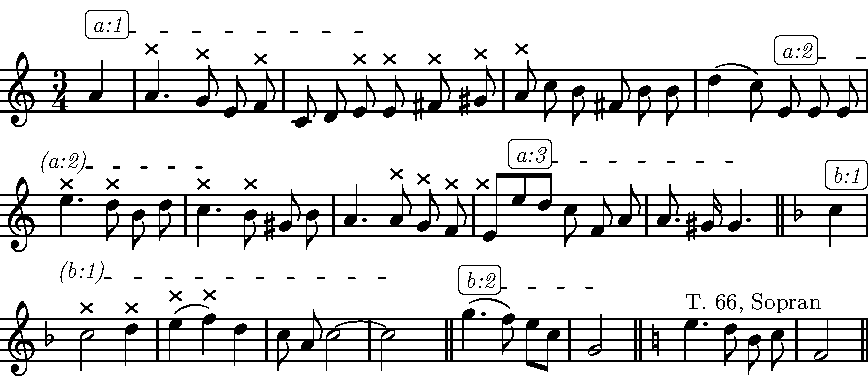
\includegraphics{nbs-my-love-motivik.pdf}
 \caption{Die Melodie der ersten Strophe von \textit{My Love dwelt…} und
 ihre motivischen Bestandteile; Motive der dritten Strophe}
 \label{nbs:my-love-motivik}
\end{notenbeispiel}

Der Unisono-Beginn des Liedes prägt mit seiner fallenden Melodik, dem
gedämpften Klang und der Tonart a-moll die Grundstimmung des Liedes:
archaisch anmutende Strenge und edle Trauer.  Das lyrische Ich ist
räumlich und zeitlich weit getrennt von den erzählten Ereignissen und
blickt mit Wehmut zurück.  Der grüne Wald (V.~2) wird weniger als Idyll
denn als Einöde empfunden, und nachdem ein dominantischer Orgelpunkt
Spannung aufgebaut hat, wird mit einem \enquote{harmonischen Rückschritt}
eine plagale Kadenz erreicht, und \textit{ritardando}, abphrasiert und mit
Fermate verebbt die Bewegung bereits im vierten Takt wieder völlig.

Die zweite Phrase hebt \textit{a tempo} mit einem Oktavsprung an, der das
\engquote{far away} erfahrbar macht und dessen Echo eine ostinate
Begleitfigur der Männer anstößt.  In den schon erwähnten zwei Tetrachorden
fällt die Melodie wieder zurück, und als sich der Oktavsprung wiederholt,
wird er durch ein neuerliches \textit{ritardando} zur bloßen Erinnerung,
die von Motiv \textit{a:3} zum Halbschluss gerundet wird.

Langs erste Strophe hat durch die Fünfzeiligkeit, ihre ungezwungenen
Jamben und starken Enjambements einen erzählenden Tonfall; dementsprechend
fallen die 4+5 Takte von Elgars Phrasen nicht mit den Textzeilen in eins,
sondern folgen den Sinnabschnitten.  Dadurch wird die zweite Strophe mit
ihrem anderen Aufbau zu einer Herausforderung, der Elgar durch subtile
Anpassungen begegnet, wie die Textwiederholung \engquote{slowly, slowly},
welche Text- und Melodiezeilen synchronisiert.

Mit der zweiten Strophe kehrt nun in die stille Landschaft Bewegung ein
und der Einbruch der Nacht führt eine magische Veränderung herbei; da passt
Elgar auch die Harmonik für die zweite Strophe an.  Ein Stimmtausch zwischen
Sopran und Tenor leitet die erste, verhaltene Wendung nach C-Dur ein; nach
der Fermate hebt die zweite Halbstrophe zwar an wie bekannt, dann aber folgt
anstelle der fallenden eine steigende Sequenz, aus dem ganzen Motiv, und
emphatisch gesteigert durch die Chromatik im Alt bricht ein strahlendes,
sechsstimmiges C-Dur hervor.  Jedoch bei Tagesanbruch fällt die Erscheinung
binnen eines Taktes in sich zusammen, und Motiv \textit{a:3} schließt sich
diesmal, mit \emph{zweimaligem} ritardando, ganz.

Die ersten beiden Strophen sind in zusammen 19 Takten vertont; für die
dritte Strophe verlässt Elgar den erzählerischen Gestus und breitet sie
in träumerischer Weite von 30 Takten aus.  Hier ist das Idyll, in der Nacht,
bei Mondenschein, und in der Natur.  Für dieses Idyll findet Elgar eine
höchst exquisite Farbe: subdominantisch-warmes, pastorales F-Dur\footnote{Moore
\parencite[S.~142]{moore} spricht von D-Dur, offenbar lag ihm eine der
Bearbeitungen für Frauenchor vor, bei denen der Mittelteil in der Tat im
Interesse reizvoller Instrumentationseffekte von Elgar nach D transponiert
ist.}, äußerst leise Dynamik, die Melodie \textit{dolcissimo}
in Oktaven verdoppelt, über einem leicht tänzerisch-pulsierenden Klangteppich
der restlichen Stimmen.  Die Harmonik ruht zunächst völlig, öffnet sich dann
im siebten und achten Takt und bereitet einen melodischen Aufschwung im
\lilyDynamics{mf} vor (wieder wird C-Dur mit Spitzenton \textsf{g}$''$ im
Sopran erreicht).  Die Sequenzierung beginnt T.~30 im \lilyDynamics{p}
bereits wieder die sanfte Rückführung zur wörtlichen Wiederholung der
herrlichen, weitgespannten Melodie.  Beim zweiten Mal aber bricht das
zweite Motiv gar im \lilyDynamics {f} heraus (gegen \lilyDynamics{pp} im
Vortakt) zur Katastrophe des \engquote{like a brand for battle drawn}, und
nach zwei ritardierenden Takten ist T.~46, \engquote{She fell, and flamed
in a wild dawn} in weich-nostalgisches A-Dur gehüllt – eine ganz neue
Farbe, an die sich aber die vierte Strophe bruchlos anschließen kann.

Diese gestaltet sich nun als eine Reminiszenz: nachdem sie wie die erste
Strophe beginnt und in T.~55–57 das C-Dur der zweiten wieder aufgreift, folgt
plötzlich in T.~58 der Beginn der dritten Strophe, in einer Variante, die
auf subdominantischem d-moll beginnt und melodisch ihren Elan eingebüßt hat:
mit dieser Musik wird preisgegeben, dass der Geliebte unter dem Gras liegt,
und der Schmerz über sein erkaltetes Herz äußert sich in einer Variante von
\textit{b:2}, deren Spitzenton scharf dissonierend und \lilyDynamics{ffz
p} hereinsticht.  \engquote{colder than the clay} klingt es am Beginn
der kurzen Coda, wenn der Tenor in tiefster Lage vom Alt in der Oktave
imitiert wird; der Sopran antwortet in der Quinte mit der bereits erwähnten
Synthese.  Vielleicht ist es nicht übertrieben, darin einen Erfolg der
Trauerarbeit zu sehen, denn die Plagalkadenz führt \textit{molto rallentando}
zu einem pikardischen Schlussakkord.  Es ist noch nicht der Elgar, der
23~Jahre später die Ode \textit{The Music Makers} in f-moll so düster
schließen lassen wird, wie er sie eröffnet hat.

\section{There is Sweet Music Here \textmd{op.~53 Nr.~1 (1907/8)}}

Seit Winter 1903/4 hatten die Elgars Italien anstelle der bayerischen
und österreichischen Alpen als bevorzugtes Urlaubsziel ausgewählt.  Schon
damals war das Ziel gewesen, ein inspirierendes Umfeld für die Arbeit an
der ersten Symphonie zu finden – jedoch erst als sie vier Jahre später
wieder in Italien waren, gelang es Edward tatsächlich, mit der Komposition
zu beginnen.  Als er einige Skizzen verfasst hatte, legte er sie im Dezember
beiseite und schrieb part-songs.  Zunächst waren das vier Werke auf Texte,
die ihm von außen angetragen wurden: \textit{How calmly the evening once
more is descending} für vierstimmigen Chor \textit{a capella}, ein
\textit{Christmas Greeting} für Frauenchor, zwei Geigen und Klavier,
ein \textit{Marching Song} (für einstimmigen Chor mit Klavier oder
Orchester) sowie \textit{The Reveille}, ein beeindruckender Männerchor
und durchaus würdiges Pendant zu Gustav Mahlers \textit{Revelge} aus
den Wunderhorn-Liedern.

Nach diesen aber schrieb er aus eigenem Antrieb vier weitere: die großen
part-songs des op.~53.  Hier war er frei in der Wahl seiner Texte, bis
dahin, dass er den Text für das vierte selbst verfasste (das Pseudonym
Pietro d’Alba bezieht sich auf Peter, das geliebte weiße Kaninchen
seiner Tochter).

\subsection*{Textwahl}
Mehrere Aspekte sind an der
Wahl der Verse von Alfred Lord Tennyson für das erste\footnote{in der
endgültigen Reihenfolge – ausweislich der Manuskripte hat Elgar
verschiedene Anordnungen erwogen.} der Lieder bemerkenswert:

\begin{itemize}
 \item Südländische Topoi als Inspiration ziehen sich durch Elgars gesamtes
 Schaffen, von der frühen Konzertouvertüre \textit{Sevillana} (1884) über
 \textit{In the South} (op.~50, 1904) – Dokument der kreativen Anregung aus
 den Italienurlauben dieser Jahre – bis hin zu den
 Entwürfen zur Oper \textit{The Spanish Lady} aus den letzten Lebensjahren.
 Tennysons \textit{The Lotos-Eaters}, aus dem Elgar hier die erste Strophe
 des \engquote{Choric Song} vertont,
 ist selbst durch eine Spanien-Reise angeregt\cite[p. 122]{ece13}.

 \item Die Handlung des Gedichts ist Homers \textit{Odyssee} entnommen und
 somit befindet sich die traumhaft-arkadische Landschaft nicht nur geographisch,
 sondern auch zeitlich in weiter Ferne.  Wenn Elgar das Stück gegenüber Ivor
 Atkins mit den Worten \engquote{It will sound very remote \& will please
 the village choirs} einführt\footnote{in einem Brief vom 17.~Januar 1908,
 zitiert in \cite[S.~169]{atkins}}, so ist die zweite Hälfte dieses Diktums
 natürlich ironisch gemeint (vergleichbare Schwierigkeiten muss man in der
 Chorliteratur vor Elgar lange suchen\footnote{W.\,G. McNaught schreibt:
 \engquote{I have been gazing at \enquote{There is sweet music} and am
 longing to hear it done by a real live choir.  It will give some conductors
 a bad quarter of an hour.} \parencite[Bd.~2, S.~693]{elgar-publ} – Die
 \textit{a-capella}-Werke von Peter Cornelius (wie op.~11, op.~18 und das
 Requiem nach Hebbel) sind in der Chorbehandlung vergleichbar und auch
 stilistisch gibt es Entsprechungen; sie scheinen sogar ein direkter
 Vorgänger zu sein: in einem Brief vom 14.~Juli 1909 zieht Elgar eine
 Parallele zwischen seinem op.~57 und Chorliedern von Cornelius.}), die
 erste Hälfte aber nennt m.\,E. einen entscheidenden Bestandteil der
 Semantik des Werks.

 \item Die elf Verse, die Elgar seiner Vertonung zugrunde legt, bilden eine
 einzige Strophe und bieten somit Gelegenheit, eine andere formale
 Architektur in das Genre des Lieds hineinzubringen.  In dieser assoziativen
 Beschreibung einer Landschaft bilden sich auch keine eigentlichen
 Handlungselemente heraus.  An Reimmuster (ABAB-CCC-DDDD) und Satzstruktur
 lässt sich eine Gliederung in $4+(2+1)+4$ Verse erkennen\footnote{Die Verse
 sind daher im Folgenden die Verse nicht als 1–11, sondern als \textit{A1–4,
 B1–3, C1–4} numeriert.}, die aber nur sporadisch eine Entsprechung in
 musikalischen Formzäsuren findet.

 \item Wie in Andrew Langs \textit{Romance}, über die wir oben sprachen, so
 sind auch hier die Jamben oft durch Gegenakzente einem freien Rhythmus
 angenähert und gerade inhaltlich zentrale Wörter wie \engquote{sweet}
 (\textit{A1}) und \engquote{still} (\textit{A3}) treten anstelle der Senkung
 auf.  Verse dieser Art gehen offenbar eine glückliche Verbindung mit Elgars
 speziellem Modus der Textvertonung ein, indem häufig zuerst eine musikalische
 Idee kommt, die in einem weiteren Arbeitsschritt gewissermaßen in den Text
 gekleidet wird.
\end{itemize}

\subsection*{Form}
J.\,P.\,E. Harper-Scott beschreibt die Grundkonzeption der ersten
Symphonie op.~55 und anderer Werke Elgars mithilfe des Begriffs der
\engquote{immuring-immured tonal structure}, d.\,h. dass das Werk zwei
tonale Zentren hat, deren eines das andere \enquote*{einmauert} und
gefangen hält.  Im Unterschied zur klassischen Sonatenform Beethovens
finden These und Antithese hier nicht zu einer Synthese und der Konflikt
bleibt ungelöst.\footnote{Für die ausführliche Darstellung dieser Theorie
und ihrer musikanalytischen und philosophischen Grundlagen siehe
\cite{harperscott2006}.}

Von einem Konflikt kann bei diesem Lied nicht die Rede sein, aber es
erweist sich in diesem Licht, dass die Gegenüberstellung von G-Dur und
As-Dur\footnote{J.~N. Moore \parencite[524]{moore} hat bereits auf die
Signifikanz dieser beiden Tonarten hingewiesen.  G-Dur (und g-moll) trat
von Beginn der kompositorischen Tätigkeit an häufig an wichtigen Stellen
auf, As-Dur ist die Tonart des \engquote{ideal call} in der ersten
Symphonie.} nicht nur kompositorischer Gedankensport ist (obgleich Elgar
ein Freund von Rätseln und ähnlichem war).  Sie ist auch Ausdruck einer
semantischen Grundidee sowie konstitutiv für die Form, indem die beiden
Tonarten die Rolle des ersten und zweiten Themas einnehmen.  Tabelle
\vref{table:sweet-mus-form} gibt eine Analyse der Form mit den
Begriffen von Hepokoski und Darcy\cite{hepokoski-darcy}.

\newcommand{\sleep}{\textrm{\engquote{sleep}}}
\begin{table}
 \centering
 \caption{
 Formübersicht zu \textit{There is sweet music}, op.~53, Nr.~1\\
 \small\textsf{Legende: Exp. Exposition – Dev. Durchführung (Development) –
 Rec. Reprise (Recapitulation) – P erstes Thema (primary) – S zweites Thema
 (secondary) – TR Überleitung (transition) – C Schlussgruppe (close) – E
 Episode – $\times$~verknüpft mit}
 }
 \begin{tabular}{l|I|C||C|I|r}
  \multicolumn{3}{c||}{Frauenstimmen}& \multicolumn{3}{c}{Männerstimmen} \\
  Takt  & Text & \multicolumn{2}{c|}{Formabschnitte}  & Text & Takt  \\
        &      & \multicolumn{2}{c|}{\textbf{Exp.} P} & A1–4 & 1–8   \\
  7–11  & A1–2 & S                   &                &      &       \\
  12–13 & B1–2 & \multicolumn{2}{c|}{TR}              & B1–2 & 13.14 \\
  14–17 &      & \multicolumn{2}{c|}{C}               &      & 15–17 \\
  18    & B3   & \multicolumn{2}{c|}{TR}              & B3   & 18    \\
  19–21 &      & \multicolumn{2}{c|}{\textbf{Dev.} E} &      & 19–24 \\
  22.23 & C1–4 & E                   &                & (C1  & 23.24)\\
  24–26 &      & E$\times$S          & E$\times$P     & C1–4 & 25–26 \\
  27    &      & TR                  &                &      &       \\
  28–35 &      & \multicolumn{2}{c|}{C}               &      & 28–31 \\
        &      & \multicolumn{2}{c|}{\textbf{Rec.} P} & A1–2 & 33–37 \\
  36–40 & C3–4!& S                   &                &      &       \\
  41–43 &      & \multicolumn{2}{c|}{C}               & C3–4 & 38–43 \\
  44–46 &\sleep& \multicolumn{2}{c|}{\textbf{Coda}}   &\sleep& 44–46
 \end{tabular}
 \label{table:sweet-mus-form}
\end{table}

Das Stück beginnt schlicht mit einer siebentaktigen G-Dur-Melodie im
Männerchor.  Die beiden Hälften dieser unregelmäßigen Periode beginnen
mit den gleichen Akkorden, die aber mit völlig verschiedener Rhythmik
an die Diktion der Wörter angepasst werden, und beim ersten Mal mit G-Dur
in Terzlage, beim zweiten Mal überraschend mit einem \textit{unisono}
\textsf{G} enden.  Für eine Weile noch grundiert von diesem ruhenden
\textsf{G} setzen die Frauenstimmen ein und übernehmen zwar wiederum die
gleiche Musik, aber noch zwei Stufen leiser, einen Halbton höher transponiert
und mit anderen textlichen Schwerpunkten.  Durch die langjährige Erfahrung,
in eine bestehende musikalische Idee den Text schlüssig einzupassen, wenn
beispielsweise die \enquote{Leitmotive}\footnote{Zur Problematik dieses
Begriffs bei Elgar siehe \cite{csizmadia}.} in den Oratorien mit immer
neuen Textabschnitten kombiniert werden, gelingt es Elgar, dass beide
Varianten hier gleich schlüssig wirken.

Anstelle einer vierten Wiederholung des Motives mit den Versen
\textit{A3.4} folgt eine Überleitung, und wie mehrfach in diesem
Stück ist der Beginn eines neuen Textabschnitts vorgezogen gegenüber
dem eigentlichen musikalischen Neuansatz.  Der 5/4-Takt verstärkt den
schwebenden Rhythmus der Musik\cite[S.~524]{moore}, der bereits zuvor
durch die vielen Überbindungen und Gegenbetonungen spürbar war.  In T.~13
berühren sich erstmals die beiden Sphären: C-Dur ist als Paralleldominante
zu As-Dur durch die Frauenstimmen eingeführt, und wird als Subdominante im
G-Dur-Umfeld der Männer übernommen. Erneut ist die gleiche Musik mit anderer
Textverteilung realisiert, wenn nun der nächste, diesmal enharmonische
Berührungspunkt in T.~14 angesteuert wird.

Was ich als Schlussgruppe klassifiziere, besteht aus drei verschiedenen Ideen:
Die Musik der Frauenstimmen scheint mit ihren zarten (\lilyDynamics{ppp}),
im besten Sinne ziellosen Dreiklangsbrechungen von As-Dur/-moll und im
Kontext der Idee von einer Musik, die \enquote{in der Luft liegt} und in
der Natur, den Klang der Äolsharfe zu evozieren, deren Saiten nur durch
den Wind im offenen Fenster sanft zum Schwingen gebracht werden.  Ein
romantisches Instrument \textit{par excellence;} es ist belegt, dass im
Haus der Elgars, Plas Gwyn bei Hereford, ab 1904 ein solches Instrument
stand\cite[p. 443]{moore} und auch, dass es mehrfach Einfluss auf Elgars
Musik hatte\footnote{W.\,H. Reed schreibt: \engquote{[It] produced a
shimmering musical sound of elfin quality, the strings being tuned to
concordant intervals; therefore the effect […] was entrancing.} und erwähnt
die Beziehung zu einer Stelle in \textit{Introduction and Allegro}, op.~47
(Studienziffer 15, T.~6–12) (\cite[S.~147f.,]{reed} zitiert nach
\cite{hepokoski-gaudery}).  Zu Elgar und der Äolsharfe siehe auch
\cite{riley-nature}.}. – In den Männerstimmen erscheint unterdessen zunächst
ein fallendes Motiv in himmlischem E-Dur und dann in T.~17 ein Viertonmotiv
aus Quinte, Ganzton und Quarte, das durch die Stimmen wandert und durch die
Vermittlung der behutsamen Harmonisierung im Alt ein gemeinsames c-moll
etabliert.  Wo nun das Überleitungsmotiv im Sopran wiederkehrt, gehen auf
der zweiten Viertel von T.~18 die Bässe emphatisch in die As-Dur-Sphäre ein
und alle modulieren gemeinsam nach Des-Dur/Cis-Dur, welches mit dem langen
Orgelpunkt deutlich einen neuen Formabschnitt markiert.

Der Mittelteil dieser Kombination von Lied und Sonatensatzform beginnt also
mit gänzlich neuem musikalischem Material; in neuerdings stabilem 4/4-Takt
wird ein eintaktiges Motiv zwischen Tenor und Sopran hin- und hergereicht,
begleitet von ebenfalls eintaktigen Harmoniewechseln, welche dem liegenden
\textsf{Des/Cis} immer neue Farben hinzufügen.  Zunächst legen sie einen
weiten Weg zurück zu einem h-moll, das auf eine wieder neue Weise den
Eindruck einer großen Distanz erweckt, bevor in T.~23 mediantisch Es-Dur
überrascht und zurück nach As-Dur führt.  Die Landschaft ändert sich
schleichend: in T.~22 beginnt der Text der dritten Teilstrophe, zunächst
in den Frauenstimmen, dann je anderthalb Takte später von Tenören und
Bässen übernommen; das Episodenmotiv erscheint erstmals im Alt als
Mittelstimme, und schließlich fällt das \textsf{Des} im Bass nach
\textsf{C}.

Im Grunde ist nun eine zweite, nicht rein episodische Phase der Durchführung
erreicht, denn während die Motivik noch unverändert bleibt, tritt die
Gegenüberstellung von G- und As-Dur und somit die Essenz von erstem und
zweitem Thema wieder auf den Plan.  Die stete Bewegung der Episodenmusik
wird in einem Überleitungstakt retardiert und so die Wiederkehr der
Schlussgruppe vorbereitet, welche nun mit dem Text der dritten Teilstrophe
unterlegt ist.  Dreimal erreichen die Frauenstimmen ein \textsf{ces} – beim
dritten Mal tut sich eine \enquote{Lichtung} auf, die Bewegung ist plötzlich
aufgehoben, und in diesem Freiraum erscheint die Musik des Beginns wieder.

Gegenüber den 17~Takten der Exposition ist die Reprise mit 11 Takten deutlich
verkürzt, quasi gestaucht.  Alle Überleitungen fallen aus und die Männerstimmen
kontrapunktieren das zweite Thema der Frauen bereits mit dem Viertonmotiv der
Schlussgruppe (T.~38f.); die Reprise des \enquote{ersten Themas} schließt
bereits nach den ersten beiden Versen im \textit{unisono} \textsf{G}, und
die Frauen antworten darauf sogar nur mit den ersten zwei Takten, die zweimal
gesungen werden, zum Text der dritten Teilstrophe: der Rückgriff auf den
Beginn des Textes war nur von kurzer Dauer.  Die Schlussgruppe schwankt
unter den \enquote*{Äolsharfen}-Dreiklängen der Soprane zwischen As-Dur,
c-~und f-moll, und die Coda geht daraus hervor, indem nur das letzte Wort
des Textes übrig bleibt und die Entfernung zwischen G-Dur und As-Dur nun
wieder gänzlich unüberbrückt ist.

\subsection*{Semantik}
Verschiedene Dreiteilungen durchdringen sich in diesem klingenden Idyll:
Die musikalische Form ist organisiert in der Dreiteiligkeit von Exposition,
Durchführung und Reprise (da die Coda viel geringeren Umfang hat).  Die
drei Teilstrophen der Textvorlage treten dazu mit ihrer eigenen Verteilung
in subtilen Dialog.  Dazu lassen sich auch in der harmonischen Anlage drei
\enquote{Modi} unterscheiden: in erstem und zweitem Thema sind die beiden
Sphären getrennt, in der Überleitungsmusik berühren sie sich, sind zu Beginn
der Durchführung ganz vereint und gestalten für sieben Takte (18–24) gemeinsam
die Harmonik.  Dann wird die Bindung wieder schwächer mit der Überleitungsmusik,
bis zum Schluss die Entfernung wieder so groß wie am Anfang ist.

Durch diese sanduhrähnliche Form erhält der mittlere Abschnitt mit dem
Satz \engquote{Music that brings sweet sleep down from the blissful skies.}
zentrale Bedeutung: Musik, die aus einer besseren, himmlischen Welt kommt
und deren Gabe süßer Schlaf, also gute Träume sind.  \engquote{sleep} steht
auch als letztes Wort des Textes und des Liedes da, bleibt in der Coda
alleine übrig und wird noch achtmal wiederholt.

Träume, oft in enger Verbindung zur Musik gesehen, sind ein Grundthema
von Elgars kreativer Tätigkeit, darauf ist oft hingewiesen worden.  In
Werken wie \textit{The Dream of Gerontius} und \textit{The Dream Children}
zeigt es sich bereits am Titel; am stärksten aber ist von dieser Thematik
die Ode \textit{The Music Makers} durchzogen, die für Elgar ein sehr
persönliches Anliegen war.\footnote{Siehe \cite[S.~631–641,]{moore} für
den engeren biographischen Kontext der Entstehung.}  Dort finden sich
Textstellen wie \engquote{We are the music makers, and we are the dreamers
of dreams}, \engquote{we with our singing and dreaming}, und viele mehr,
und sind gekleidet in eine düstere, melancholische Grundstimmung.  Die
\textit{Music Makers} identifizieren sich gleich in der ersten Strophe als
\engquote{world-losers and world-forsakers}, und zumindest in Elgars
Interpretation aus dem Jahr 1912 geht diese Weltflucht mit großer Wehmut
einher.

Nicht so in \textit{There is sweet music}: Hier sind die Götter gnädig
gestimmt und wer diese Musik und diese Landschaft erlebt, empfängt echte
Seelenruhe und \engquote{sweet sleep}.

\section{They are at Rest \textmd{(1909)}}
Eine paradiesische Vision ganz anderer Art wird in diesem kurzen Anthem
entfaltet.  Äußerlich unterscheidet es sich in fast jeder Hinsicht: Es
handelt sich um ein Auftragswerk, von Walter Parratt als Master of the
King’s Music für den neunten Todestag\footnote{22. Januar 1910; Michael
Kennedy spricht irrtümlich vom \engquote{tenth anniversary} \parencite
[S.~114]{kennedy-life}.} von Queen Victoria bestellt; der Text ist
geistlich und umfasst zwei kurze Strophen; die Musik enthält nichts
von den harmonischen Kühnheiten des op.~53 und ist vorwiegend vierstimmig
gesetzt, mit gelegentlichen Teilungen.  Jedoch in der Textwahl hatte Elgar
wiederum ziemlich freie Hand; es war für einen so staatstragenden Anlass
sicher nicht selbstverständlich, aber seine Wahl eines Textes des Katholiken
Cardinal Newman wurde genehmigt.  Erneut handelt es sich hier um einen Text,
dessen poetische Form mit Unregelmäßigkeiten in der Zeilenlänge und im
Rhythmus der zweiten Strophe nicht allzu fest gestrickt ist.

\subsection*{Motto}
Elgar gewinnt aus der ersten Zeile nicht nur den Titel des Werks, sondern
setzt sie zusätzlich als eine Art Motto ein, das zu Beginn und Schluss je
zweimal wiederholt wird, einmal affirmativ und einmal retardierend,
echoartig.  Der Parallelismus der Dynamik wird überlagert von einer
chiastischen Motiventsprechung; das zweite Glied des Beginns wiederholt
der Schluss als erstes Glied fast wörtlich, nur mit etwas gedämpftem
Impetus durch die fehlende Punktierung und die zusätzlichen Sextenparallelen
zwischen Sopran und Tenor.

Das zweite Glied der Coda weist eine Ähnlichkeit in der Bewegung zum
ersten Glied des Beginns auf, die sich aber kaum näher bestimmen lässt,
da die Harmonik umgekehrt ist: paradoxerweise fällt es am Beginn direkt
von Fis-Dur nach h-moll, während der Schluss sich wieder nach Fis-Dur
öffnet – allerdings nicht in einer plagalen Kadenz; der eingeschobene
Quartsextvorhalt auf \textsf{cis} konstituiert eine authentische
Kadenz und qualifiziert das Fis-Dur, dem Wortsinne von \engquote{rest}
entsprechend, als Tonika.  \textsf{Cis} wirkt nicht als
\textit{Zwischen}dominante, da die überraschende Wirkung durch
die wohl recht starke Verlangsamung (\textit{Più lento, dim. e
rit.} \underline{und} Tenutostriche) aufgehoben wird.  Dennoch
steckt eine Öffnung in diesem Schluss – vielleicht ist in der
\enquote*{Paradoxie}\footnote{griechisch: entgegen/quer zur
Erwartung/(Welt-)Anschauung} umgesetzt, dass diese Ewigkeit
\enquote*{jenseits unseres Erfahrungshorizontes} liegt.

\subsection*{Satztechnik und Formverlauf}
Das Motto ist abgesetzt durch klare homophone Setzweise, während in den
Strophen die Unterstimmen viele eigene rhythmische Impulse setzen; direkt
mit Beginn der Strophe ist es der Bass, der das Geschehen belebt, und in
T.~5 antwortet das \textsf{cis} der Tenöre auf den Sopran.  Am Ende von
T.~4 stellen Alt und Tenor Hörner dar, welche eine Steigerung einleiten,
in der Melodie durch einen Stufengang \mbox{\textsf{h-cis-d-e}} umgesetzt.
Es ist reizvoll, davon auszugehen, dass sich \textit{diminuendo} und die
Gabeln Ende T.~6 auf verschiedene Ebenen der Ausführung beziehen: die
Gabeln (welche traditionell nicht unmittelbar die Dynamik bezeichnen\cite
[Kapitel 1]{poli}) bestätigen, dass das Phrasenziel die Eins von T.~7
ist, während das \textit{diminuendo} ebenso wie das \textit{crescendo}
einen Takt zuvor die Wörter \engquote{rude}, \engquote{prayer} und
\engquote{waywardness}\footnote{\engquote{wayward} meint hier eigensinnig,
launisch.} illustrieren.  Wirkungsvoll eingesetzt ist auch die Homophonie
auf \engquote{heav’n of their repose} und \engquote{prayer}.

Durch ein neuerliches \textit{rit.} vorbereitet, beginnt \textit{Tranquillo}
die zweite Hälfte der Strophe mit einer der personalstil-typischen Sequenzen,
die sich bogenförmig über die T.~8–10 erstreckt.  Ihre Oberstimme ist aus dem
Motiv des zweiten Taktes gewonnen, welches als Keimzelle das ganze Stück
hindurch wiederkehrt.  Der Schluss der Strophe ist mit einem langen Melisma
von erhaben fließenden Vierteln gestaltet, frappierend ins Relief gesetzt
durch die vorhergehenden lebhaften Sechzehntel.  Elgar wird dabei vor allem
an das \engquote{chant} der zweiten Strophe gedacht haben.

Zu Beginn dieser zweiten Strophe greift der Komponist für den Kurzvers
\engquote{And soothing sounds} auf die Musik des Mottos zurück und knüpft
sie, entsprechend dem Enjambement, an die folgende Phrase an.  Das Gerüst
der ersten Strophe ist komplett beibehalten, aber im Detail finden sich in
jedem Takt subtile Anpassungen, um die rhythmischen und inhaltlichen
Schwerpunkte der Worte getreu zu realisieren.  Die eng’lischen Wächter
der Einfriedung des Paradieses treten im \lilyDynamics{f} hervor, ihre
Gesänge hallen durch die Landschaft so zart wie das Murmeln des Flusses
in der ersten Strophe.

\subsection*{Harmonik}
Der erste Takt des Stückes kadenziert stabil nach h-moll; nachdem diese
Stabilität aber im zweiten Takt gleich wieder aufgelöst wird, gibt es im
ganzen Verlauf keine Gelegenheit mehr, von h-moll als einer Grundtonart
zu sprechen.  Die einzige eigentliche authentische Kadenz ist nach einem
terzweisen Anstieg über h-moll – D-Dur – fis-moll die nach A-Dur im vierten
Takt der Strophe, doch dieses löst sich nach D-Dur wieder auf.  Die zweite
Hälfte der Strophe changiert dann wieder zwischen h-moll und D-Dur.

John Butt hat auf die Bedeutung von Elementen der Modalität und gregorianischer
Tradition für Elgars früheste musikalische Erfahrungen hingewiesen:
\label{butt:1}\engquote{[I]t may be worth considering what the influence
of chant and modal melodic and harmonic thinking might have been on a
composer who assimilated so many things intuitively, with little formal
training.  He clearly had no difficulties in absorbing the indigenous
English sentimental style, with its roots in the foreigners, Handel, and
Mendelssohn, and developed to a level of passable excellence by S.\,S.
Wesley, Sullivan, and Parry.  What rendered him outstanding was his
mastery of the most advanced compositional technique of the Germanic
tradition.  If one were to imagine these two traditions tempered –
almost unwittingly – by the tonal ambiguity generated by Gregorian
chant, it is not entirely implausible to imagine a style that is
traditionally English, technically excellent, and up-to-date, yet
tinged with a melodic, tonal, and harmonic ambiguity, something that
could be heard as nostalgic ineffability, an underlying uncertainty
and melancholy.\cite[S.~107f.]{butt-rcath}}
Insbesondere der letzte Satz passt nahezu perfekt auf die Faktur und Stimmung
von \textit{They are at Rest}.  Traditioneller, liedhafter Duktus sowie
raffinierter Umgang mit Satztechnik und Form verbinden sich mit der
ästhetischen Wirkung dieser speziellen Form von modaler Harmonik, und
tragen dazu bei, dass die Musik Ausdruck sowohl von Newmans Vision als
auch von Elgars künstlerischem Befinden wird.

Bei näherer Betrachtung ist nämlich die Botschaft des Textes alles andere
als harmlos: Zum einen wird das Paradies weniger als ein Ort des Glücks
oder Genusses, sondern vielmehr einer stoischen Gelassenheit und Indifferenz
gezeichnet, zum anderen sind diese Heiligen vom irdischen Schicksal der
Nachgeborenen vollkommen abgewandt und es wird gar als Affront bewertet,
sie mit Gebeten zu behelligen.

Dass Cardinal Newman als herausragender Vertreter des Katholizismus seiner
Zeit (zumindest in England) solche Empfindungen äußert, ist symptomatisch
für die Krise des Glaubens in der Moderne, und gerade deshalb steht es
Elgar besonders nahe.  Womöglich katalysiert durch die Arbeit an der in
vielerlei Hinsicht unvollendeten Oratorientrilogie hatte er in den Jahren
ab 1901 seinen Glauben weitgehend verloren\cite[Zu Elgars Verhältnis zur
Religion siehe][]{adams, rushton-religion}.  Es zeugt auch von seinem
Geschick im Umgang mit gesellschaftlichen Erwartungen, oder von einer
Fähigkeit zur Selbstverleugnung, oder vom Selbsterhaltungstrieb des
von öffentlichem Wohlwollen abhängigen Komponisten, dass es ihm gelang,
diese gefährliche Botschaft unter der Oberfläche eines schönen Anthems
zu verbergen.

\section{Go, Song of Mine \textmd{op.~57 (1909)}}
Bei diesem Werk kommen verschiedene disparate Elemente zusammen: Elgar
vertont einen nichtliturgischen lyrischen Text für unbegleiteten Chor;
die Aussage ist aber eindeutig und ungebrochen geistlich, und die Setzweise
und Emphase des Ausdrucks haben symphonische Ausmaße, die sich in Elgars
\textit{a-capella}-Musik zuvor nicht finden ließen.  Entsprechend lässt
sich das Werk schwer in ein Genre einordnen; die Erstausgabe bezeichnet
das Stück nicht als part-song, sondern als \engquote{Chorus (unaccompanied)
in six parts} und wurde im Format eines in Papier gebundenen Oratoriums (!)
gedruckt\cite[Brief an A.~H. Littleton vom 27.~Juni 1909, in][Bd.~2, S.~724]
{elgar-publ}. In der Elgar Complete Edition ist es in Bd.~13\cite{ece13}
unter die weltlichen \textit{a-capella}-Chöre eingeordnet, eine diskutable
Entscheidung.

Die Textvorlage besteht aus sieben Versen im Reimschema \textsf{ABBACCA},
welches intrikat eine symmetrische Anlage um drei Säulen herum mit der
klaren Hinführung auf das Ziel des \engquote{heavenly shrine} verbindet.
Inhaltlich wird ein großer Kontrast gezeichnet zwischen irdischem Leben
und himmlischer Herrlichkeit, aber gerade im hiesigen Schmerz sieht
Cavalcanti einen Weg vorgezeichnet, der ohne Zweifel zur Erlösung führt.

Es zeigen sich also größte Diskrepanzen zum hoffnungslosen Anthem \textit{They
are at rest}; eine Gemeinsamkeit liegt aber in der Art, wie Elgar die formale
Anlage des Textes modifiziert, indem er den Beginn als ein Motto herausgreift
und die Vertonung damit umrahmt.

Ein feierlicher (\textit{solenne}) h-moll-Akkord eröffnet die Komposition;
eine Anrufung des ganzen Chores, der zunächst kantillierend verweilt, dann
plötzlich Fahrt aufnimmt und nach dem Höhepunkt den Bogen wieder schließt.
Aus der Ruhe heraus tritt der Tenor, der \textit{quasi recit.} die Worte
wiederholt und wiederum eine Fermate in tiefer Lage erreicht.  Ganz versteckt
sind in die Begleitung im zweiten Alt die ersten fünf Melodietöne erneut
verwoben.

In einem für Elgar typischen Kunstgriff werden die eröffnenden neun Takte in
der Mediante wiederholt; er unterlegt sie nun mit der ersten Aussage dieses
Gesangs, den das lyrische Ich an den Menschen ausschickt: Von Staub zu
\emph{Staub} kehrst du zurück.  Beginnend in fahlem es-moll, moduliert die
Musik beim zweiten \engquote{dust} schockartig und allmählich klärt sich die
Harmonik nach d-moll, von wo wiederum die Tenöre ihr Rezitativ beginnen.

Nach diesem schlägt von dem liegenden a aus die Stimmung um, und es folgt die
zweite, verheißungsvolle Aussage dieses Gesanges im Gesang, kontrastierend
zum Beginn wie ein zweites Thema (eines Beethoven’schen Sonatensatzes), in
der Tonart und der Melodik, die nun von aufwärts gerichteten Sprüngen geprägt
ist.  In diesem zweiten Thema bildet der erste Takt eine Art Präfix, gefolgt
von einem Kopfmotiv in zwei Wellen sowie einer sequenzierenden Fortspinnung,
in der Sopran und Alt sich über resoluten Bassschritten abwechselnd in die
Höhe schrauben.  Sowie die Sequenz noch ausläuft, verschränkt sie Elgar schon
mit dem Präfix, um die gesteigerte Wiederholung des Themas vorzubereiten.

Diese Steigerung führt zu einem neuen Abschnitt, der \lilyDynamics{ff}
bereits beginnt und zu den Worten \engquote{being purified} über einem
ostinaten viertönigen Basszug unzweideutig Wagners Musik zu Isoldes
Liebestod anklingen lässt.\cite[p.~553]{moore}  Das ist zwar zunächst
sicher durch den grandiosen, hingebungsvollen Affekt motiviert, den Elgar
hier anstrebt, aber vielleicht ist die Erlösung durch eine göttliche Macht
ein semantischer Anknüpfungspunkt, der ebenso passend erscheint.  Dreimal
wiederholt Elgar die zwei Takte in genial orchestriertem Stimmentausch, um
im \lilyDynamics{fff} das Ziel \engquote{To seek its Maker at the heav’nly
shrine} zu erreichen.  Die melodiöse, breit gezogene Kontrapunktik wird
durch ein homophones, impulsives Skandieren abgelöst, überstrahlt von den
Sopranen, die in weit gespanntem Bogen über neun Takte hinweg langsam um
eine Oktave absinken, von der Mitte an durch die Baritöne in der Unteroktave
begleitet.  Nach wiederum drei sequenzierten Wiederholungen sinkt die Musik
von as-moll über fis- nach e-moll, zugleich über \lilyDynamics{p} ins
\lilyDynamics{pp}, und es beginnen sich die formalen Bögen zu schließen.
Die ostinate Motivik des \engquote{being purified}, welche zuvor in
sehnsuchtsvoller Erwartung zwischen Subdominante und Tonika pendelte,
wird nun eine Quarte tiefer und \lilyDynamics{p}~\textit{dolcissimo}
noch zweimal aufgegriffen.  Indem sie nun sich von Tonikasextakkord zu
Dominantsextakkord öffnet, äußert sie zum Einen die Erleichterung, die
kommende Erlösung geschaut zu haben, zum anderen erlaubt es Elgar, den
letzten Klang als Fis-Dur zu reharmonisieren.

Mit diesem Fis-Dur entschwindet die Musik in der Ferne, und es ist nun die
Erkenntnis vorbereitet, dass die gesehene, gleißende Zukunft noch nicht hier
ist; diese Erkenntnis kommt gekleidet in die Musik des Anfangs, welche fast
wörtlich wiederholt wird.  Der Schluss der ersten Phrase wird dabei durch
die noch schmerzlichere Vorhaltsdissonanz in T.~54 (verglichen mit T.~5)
gedehnt.  Zuletzt, wo aus dem Rezitativ der Tenöre das einzelne \textsf{fis}
übriggeblieben ist, sendet Elgar die Botschaft des Liedes noch mit einem
getupften, leisen H-Dur-Akkord wie mit einem Segenswunsch hinaus:
\engquote{Go, song of mine!}

Im Vergleich beispielsweise mit \textit{They are at Rest} ist es erstaunlich,
zu sehen, welch großes Pfund Hoffnung in diesem gewaltigen Spruch steckt.
Für die kompositorische Umsetzung des Verhältnisses zwischen dem irdischen
Leid und der himmlischen Verheißung setzt Elgar hier erneut eine Form von
\engquote{immuring-immured tonal structure} ein.  Zwar ist das Modell hier
in gänzlich anderer Weise umgesetzt: die beiden Tonalitäten sind ganz
klassisch als Parallelen aufeinander bezogen; ihre Begegnung ist nicht
als hartes Aufeinanderprallen, sondern mit weichen harmonischen Übergängen
gestaltet; und der Rahmen wirkt (wenn die Assoziation überhaupt angebracht
ist) wie ein \enquote{Sonatensatz ohne Durchführung und ohne Reprise}.  Aber
gerade das ist bezeichnend: der Kontrast wird exponiert, und nach der breiten
Schilderung der Aussicht in den Himmel folgt direkt eine Coda; durch das
Fehlen von Durchführung und Reprise entfaltet sich kein Dialog, an dessen
Ende bereits eine \enquote{Lösung} steht, noch wird eine Reise erzählt,
die zum Ziel führt – obwohl eine solche Lesart der Textvorlage durchaus
naheliegend gewesen wäre.

Doch zu solch einer ungebrochenen Äußerung naiven Glaubens ist Elgar mit
seiner Lebenserfahrung nicht in der Lage; es bedarf bereits der Anregung
durch die alte Botschaft des Textes und durch die Schönheit Italiens, um
überhaupt noch in eine ferne, gute Zukunft zu blicken.  Das Ende der
Komposition zeigt den Menschen noch seinem irdischen Los verhaftet; dass
dennoch in der Vision, die sich dazwischen auftut, eine starke, tröstende
Perspektive auf kommende Erlösung gegeben ist, macht dieses Werk im Kontext
von Elgars Schaffen so bemerkenswert.

\section{Serenade \textmd{op.~73 Nr.~2 (1914)}}
Neben dem spektakulären, ja bombastischen Gemälde von \textit{Love’s Tempest}
op.~73 Nr.~1 neigt die zarte Seelenäußerung der \textit{Serenade} etwas in
den Schatten gestellt zu werden: J.~N. Moore\cite[S.~661.  Moore irrt sich
mit der Tonart des Stückes – lag ihm womöglich eine Bearbeitung für Frauen-
oder Männerchor vor? Der umgekehrte Fall war ihm bereits bei der Besprechung
von \textit{The Reveille} op.~52 unterlaufen, wo er die Version für gemischten
Chor bespricht, obwohl das Stück zuerst für Männerchor geschrieben ist.
Allerdings verzeichnet die Gesamtausgabe keine solche Bearbeitung.]{moore}
beschreibt beide Lieder in äußerster Kürze, Donald Hunt aber erwähnt das
zweite in seinen einführenden Texten in Bd.~13 der Gesamtausgabe\cite{ece13}
mit keinem Wort.  Dabei ist die \textit{Serenade} keinesfalls weniger
ausdrucksvoll, und in der Reduziertheit der musikalischen Mittel steht
sie wohl nur wenigen Werken Elgars an Modernität nach.

\subsection*{Textvorlage}
Das Gedicht\footnote{Der Besprechung liegt nur die englische Version (siehe
Anhang \vref{poem:serenade}) zugrunde.} beginnt mit einer Art Epigramm, das
in drei knappen Versen von \enquote{allzu kurzen Träumen, Träumen ohne
Kummer} spricht und das unbarmherzige Verdikt ihrer Vergänglichkeit
ausspricht.  Auf diesen unpersönlichen Beginn folgt die Beschreibung
düsteren Wetters und kahler, im Winde schwankender Bäume, ein Anblick,
in dem das lyrische Ich sein Inneres und seinen Schmerz (\engquote{pain},
V.~15) gespiegelt sieht.  Die zweite Hälfte der Strophe wird noch
persönlicher mit einer Anrede an die schlafende Geliebte/den schlafenden
Geliebten und beschwört den Schutz der \enquote{frohen Träume}.

Die zweite Strophe konkretisiert den Kontrast zwischen Traum und Welt:
Die Seligpreisung ergeht an den, der in der Lage ist, sich vor dem
nahenden Herbst und den Gefängnismauern in Träume zu flüchten – eine
wahrhaft antiheroische, desillusionierte Aussage – und wird dem
\enquote{Wehe} quälender Schlaflosigkeit gegenübergestellt.  Das
Reimschema \textsf{AAF—BCBCBF—DEDEDF} deutet mit seinen Verknüpfungen
über die Strophen hinweg an, dass die letzten beiden Strophen nur eine
inhaltliche Entfaltung und Illustration der ersten sind.  Diese inhaltliche
Klammer wird zu einer Grundidee der Musik.

\subsection*{Musik}
Elgar verwendet wieder, wie in \textit{They are at Rest}, ein Motto, um
zwei Strophen zu umrahmen, und findet dieses hier in der emblematischen
ersten Strophe bereits vorgeprägt.  Aus dem minimalen Material einer
melodischen Terz und harmonischer Quintschritte gewinnt Elgar die Musik
und lehnt sich an die Struktur der Strophe eng an: Das Motto beginnt mit
zwei kurzen, eintaktigen Gliedern, echomäßig abgesetzt, in welchen ein Pendel
zur Oberquinte ausschwingt.  Die zwei Takte des dritten Glieds bestehen aus
einem vollständigen, leitereigenen Quintfall und sind durch hemiolische
Betonungen zusammengehalten. – Die aeolische Färbung des g-moll nivelliert
harmonische Spannungen und lässt die D-Dur-Akkorde umso deutlicher
hervortreten.

Die Rhythmik des Mottos wie auch der Fortsetzung als Begleitfigur ist
konsequent homophon gehalten und bekommt durch den vorgeschriebenen Wechsel
zwischen \textit{tenuto} und \textit{staccato} eine große Prägnanz.  Dieser
artikulatorische Kontrast wird noch verschärft mit dem Legato-Seufzer in
T.~10 und den Pausen im Takt darauf, die hemiolische Betonungsverschiebung
erscheint in T.~8f. wieder und gibt der rhetorischen Frage \engquote{Why
should you scatter them in vain?} Nachdruck.  Es kann als kongenial
bezeichnet werden, wie Elgar hier eine quasi instrumental wirkende\footnote{In
einem Brief an Henry Clayton, Verlagsmitarbeiter bei Novello, erwog Elgar,
eine Bearbeitung für \engquote{small orch[estra]} anzufertigen \parencite
[Bd.~2, S.~778]{elgar-publ}.} Begleitung schafft, deren Sprachrhythmus
trotz der einfachen binären Rhythmen vollkommen natürlich ist und dem
Wortausdruck wie angegossen passt.

Vorbereitet durch eine Wiederholung der ersten beiden Takte, echomäßig
im \lilyDynamics{p}/\lilyDynamics{pp}, setzt zu T.~7 mit einer klagenden
kleinen Sexte die Melodie des Soprans ein.  Elgar stellt die unpersönlichen
Sentenzen der Unterstimmen im artikulierten \textit{parlando} und die
persönliche Betrachtung und Anrede des Soprans im \textit{legato cantabile}
gegenüber; auch in Text (der Unterchor greift bereits auf die Verse 8 und
9 vor) und Dynamik sind die zwei Ebenen deutlich unterschieden.  Die ganze
Strophe ist in drei Abschnitten zu je zwei Versen vertont; alle drei sind
durch eigene Tonarten – g-moll, Es-Dur, es-moll – charakterisiert und
bestehen aus je zwei identischen melodischen Elementen (lediglich der Schluss
des dritten Abschnitts ist abgewandelt).  Zuerst sind die Phrasen zweitaktig,
dann werden sie durch \lilyDynamics{f}-Einwürfe des \engquote{Dreams all too
brief} und \engquote{Dreams without grief} auf je drei Takte erweitert und
der dritte Abschnitt, wenngleich \textit{più mosso}, besteht aus viertaktigen
Phrasen.

Durch den Einschub von T.~13 wird die dreizeilige Naturbeschreibung
abgeschlossen und erweckt schon beinahe den Eindruck, die Strophe sei
vorüber; im Nachhinein erkennt man ihn als retardierendes Element zur
Vorbereitung der zärtlichen Anrede, die folgt.  Nach dieser fällt die
Musik wieder zurück nach g-moll mit dem zweiten Einwurf, und etwas an
dieser Konstellation scheint zu bewirken, dass das Es-Dur von T.~15
bereits wieder vergessen ist, wenn in T.~17 es-moll zum Vorschein kommt.
Die Klänge stehen trotz ihrer physischen Nähe vollkommen getrennt
voneinander und das es-moll tönt \lilyDynamics{ppp} wie aus weitester
Ferne, wie ein Schatten.  Obwohl es frohe Träume (\engquote{glad dreams})
sind, werden sie als ein Spuk (\engquote{haunt}) erlebt; der Moment ist
kostbar, aber zerbrechlich, schutzbedürftig.

Der nächste Satz wirkt in der Vertonung nahezu dissoziiert.  Liest man
ihn als Ganzes, ist er harmlos: \enquote{warum solltest du die frohen
Träume ohne Not zerstreuen?}  In diesem unheilsvollen Kontext aber
verselbständigt sich das \engquote{in vain} und führt die Unausweichlichkeit
des Schicksals und die \textit{vanitas} vor Augen.  Musikalisch setzt
Elgar diesen Schockmoment und die Dissoziation um, indem dem aufgetürmten
Ces-Dur-Sextakkord unvermittelt ein D-Dur-Septnonakkord folgt, wiederum
physisch direkt benachbart – die beiden Oberstimmen bleiben auf dem
\enquote{gleichen} Ton –, aber doch weit entfernt.  Die Art, wie das
es-moll in diesem Lied eingekapselt ist und ohne jegliche Vermittlung
in das g-moll-Umfeld eingefügt, stellt einen Extremfall der
\engquote{immuring-immured tonal structure} dar.

Der äußerst schmerzhafte Nonenvorhalt, der die Erkenntnis der Vergänglichkeit
spürbar macht, löst sich \textit{[molto] dim.} auf, das \textsf{d} der
Soprane bleibt in einer Fermate allein liegen, und dann beginnt \textit{tempo
primo} die wiegende Figur des Mottos von neuem.

In den Unterstimmen ist die zweite Strophe bis einschließlich T.~37 Note
für Note identisch\footnote{Die gelegentlich abwesenden Staccatopunkte
zählen wohl tatsächlich zu den seltenen Druckfehlern der Novello-Ausgaben.},
in ihrer Ostinato-Funktion behalten sie auch denselben Text.  Auch die
Melodiestimme bedarf hier nur geringer Änderungen, um dem Text der neuen
Strophe angepasst zu werden.  Die einzige auffällige Variante ist das
\textit{poco rit.} in T.~36: vielleicht ein Symptom größerer Entkräftung,
oder Geste des Defätismus gegen \engquote{freedom’s rescuing}.  Das
\textit{più mosso} wird diesmal durch ein \textit{accel.} vermittelt
und wirkt im Relief noch etwas stärker durch die vorherige Verlangsamung.

Nun wird die es-moll-Musik mit dem Weheruf über den von Schlaflosigkeit
Geplagten unterlegt, erhält eine Schärfe in der Diktion durch das
\textit{staccato} auf der ersten Note und einen Akzent für die erneute
Referenz auf die Vergeblichkeit des Tuns.  Auch der Höhepunkt mit der
schneidenden Kollision der Tonarten wird in dieser Strophe agogisch
vorbereitet: \textit{molto allargando} wird der Schmerz angebahnt,
welcher wie zuvor rasch wieder der tristen Grundstimmung weicht.

In der abschließenden Wiederholung des Mottos verebbt die Bewegung in
einem langen \textit{rit.}; der pikardische Schlussakkord ist nach dieser
Darstellung von Hoffnungslosigkeit und in dieser tiefen Lage kein Zeichen
von Aufhellung, sondern mehr von Schicksalsergebenheit.

Es ist bereits beschrieben worden, wie Elgars Chorlieder op. 71–73,
entstanden im Januar 1914, wie eine düstere Vorahnung der kommenden
weltgeschichtlichen Katastrophe wirken.  Nostalgie war seit jeher Teil
seines Grundbefindens gewesen, und wie nun sich ein abnehmendes Interesse
an seinen Kompositionen bemerkbar machte (z.\,B. in der kühlen Rezeption
der 2.~Symphonie) und der Tod immer öfter Lücken in sein privates Umfeld
riss, steigerte sich auch sein Gefühl der Isolation.  In der \textit{Serenade}
äußert sich diese biographische Situation in einer fast radikalen Schlichtheit
der Form und weitgehend eintönigen Bewegung.  Die teils sehr geringen Umfänge
der einzelnen Stimmen (Sopran d$'$–es$''$, Alt a$^0$–g$'$, Tenor f$^0$–c$'$,
Bass (G)B–g$^0$) entsprechen der untermodulierten Sprachmelodie des Depressiven
– Phasen depressiver Niedergeschlagenheit ziehen sich durch Elgars gesamtes
Leben.  Nur in der Kunst lässt sich dieses Empfinden nach außen tragen, und
Minskijs Verse, vermittelt durch Rosa Newmarch, gaben den Anlass zu einer
kristallin-reinen Verkörperung dieses Aspekts seiner Persönlichkeit.

\section{I Sing the Birth \textmd{(1928)}}
Eins der Werke, mit denen er das Schweigen der ’20er Jahre brach, entstand
1928 nach der Rückkehr vom Gloucester Festival\footnote{dort wurde unter
anderem Zoltan Kodálys \textit{Psalmus Hungaricus} und \textit{Le Roi David}
von Honegger gegeben \parencite{gloucester}}: ein Carol\cite[S.~777]{moore}
auf den Text \engquote{I sing the birth was born tonight} von Ben Jonson
(1572/3–1637).

\subsection*{Tradition}
Diese Komposition zeigt in mehrerer Hinsicht ein bemerkenswertes Verhältnis
zur Tradition der Gattung:

\begin{itemize}
 \item Die Textvorlage entstand, als die erste, spätmittelalterliche Blütezeit
 des Carols infolge der Reformation bereits vorüber war.\footnote{Die
 Ausführungen zur Gattung beruhen auf \cite{carol}}  Jonsons Verse entsprechen
 durch ihre schlichte Form zwar den volkstümlichen Ursprüngen, gehen aber durch
 ihre theologische Dichte weit darüber hinaus; legendenhafte Ausschmückung der
 Weihnachtsgeschichte ebenso wie Bezüge zu Heiligen bleiben aus, stattdessen
 werden unter sparsamer Anknüpfung an die biblische Handlung christologische
 Dogmen in geistreiche poetische Form gekleidet.

 \item Die Refrainstruktur, entscheidenes formales Charakteristikum des Carol,
 entsteht durch \enquote{Alleluia}-Rufe, welche auf jede Strophe antworten;
 Elgars Strophen umfassen mit nur drei Zeilen je nur eine Hälfte von Jonsons
 Strophen.  Entsprechend den frühesten Beispielen wird das Stück auch durch den
 \enquote*{Kehrvers} eröffnet.
\end{itemize}

Im 19. Jahrhundert waren die spezifischen Bedingungen der mittelalterlichen
Gattung des Carol weitgehend vergessen; \engquote{carol} war zu einem
Oberbegriff für Weihnachtslieder aller Arten geworden.  Dem gegenüber erwachte
zu Beginn des 20. Jahrhunderts ein Bedürfnis, zu den Wurzeln zurückzukehren;
beispielsweise veröffentlicht Richard Runciman Terry 1912 eine Sammlung mit
zwölf neukomponierten Carols, von denen elf auf Texte des 14. Jahrhunderts
zurückgreifen.  Sein Vorwort erklärt, dass das erste Stück der Sammlung (auf
einen zeitgenössischen Text) daher eher als \engquote{christmas song} zu
gelten habe, und nennt darüber hinaus folgende zwei Eigenschaften als
wesentlich für das Carol:

\engquote{Christmas words do not make a carol out of what would otherwise
be a hymn tune or part-song.  In other words, a tune can only be termed a
carol the nearer it approximates to the folk-song type and the further it
departs from the hymn tune.  It ought, moreover, to stand on its own melodic
basis independent of harmony.\cite[preface.]{terry}}

\noindent Beide diese Forderungen sind bei Elgar erfüllt:

\begin{itemize}
 \item Die ersten drei Strophen werden von unbegleiteten Einzelstimmen
 vorgetragen.  Damit beweist Elgar noch größere Eigenständigkeit der
 Melodie als Terry, welcher auch die solistischen Passagen durch
 Orgelbegleitung harmonisch unterfüttert.  Darüber hinaus entspricht
 der Wechsel zwischen Solo und Tutti der responsorialen Struktur, welche
 das Carol bereits von seiner tänzerischen Vorgängerin, der \textit{carole}
 in Frankreich, geerbt hat.

 \item Der volkstümliche Gestus, welchen Terry beschreibt, ist bei
 Elgar vor allem durch die schlichte Rhythmik und die modale Harmonik
 umgesetzt (die Melodie besteht ausschließlich aus den Tönen des aeolischen
 Hexachords)\footnote{Es scheint sich dennoch um eine Neuschöpfung Elgars zu
 handeln; sie findet sich nicht unter den in \cite{hymnary} verzeichneten
 Melodien, darunter eine Vertonung von Arthur Sullivan}.  Wir hatten oben
 bereits betrachtet, wie Modalität zu den frühesten Einflüssen in Elgars
 Tonsprache gehört (Abschnitt \vref{butt:1}); in direkter Fortsetzung
 unterscheidet John Butt allerdings zwischen zwei Arten modaler Harmonik:
 \engquote{Modal elements were, of course, to become central to the
 rediscovered Englishness of Vaughan Williams and his contemporaries,
 but these were acquired through conscious study of the folk and Tudor
 repertory—a completely different route from Elgar’s.}
 Es scheint, dass Elgar in seinen letzten Lebensjahren bisweilen die Distanz
 zu Ralph Vaughan-Williams und anderen Zeitgenossen der jüngeren Generation
 überwinden konnte; ein ähnlich modal geprägtes Carol finden wir beispielsweise
 im ersten Abschnitt der \textit{Fantasy on Christmas Carols} (1912) von
 Vaughan-Williams\cite{vaughan-williams} – vergleichbar auch in der
 responsorialen Anlage mit Solist und in der Gliederung durch kurze Einwürfe
 des Chores.

 \item Eine Besonderheit von Elgars Vertonung besteht in den rhythmischen
 Anpassungen von Strophe zu Strophe, durch die mit bescheidenen Mitteln
 eine große rhetorische Prägnanz erreicht wird.  Man möchte darin die
 Fortsetzung der oben beschriebenen stiltypischen Flexibilität in der
 Vertonung von Gesangstexten sehen, gäbe es nicht eine frappierende
 Entsprechung zu folgender Beschreibung: \engquote{[E]ssentially the
 novelty of the Tudor carol is its very careful attention to the sounds
 of words and the shape of short word-groups, attention so detailed that
 it was thought necessary to write out at length the verses even of
 strophic carols, with the most minute notational variations required
 for each different set of words.\cite[S.~170]{carol}}  Es wird nicht
 zu klären sein, ob Elgars Sorgfalt ihn zu solch tiefgreifender Kenntnis
 des frühen Repertoires geführt hat, oder es sich um Zufall handelt, aber
 besser könnte man nicht beschreiben, wie Elgar die Melodie den Worten
 anpasst.  Nicht nur ist in jeder Strophe der Wechsel von geraden Vierteln
 mit Punktierungen anders gestaltet, auch jedes einzelne der sparsam
 eingesetzten \textit{tenuti, staccati} und Akzente ist ideal der Diktion
 angepasst; genau so die prägnante Pause in T.~58.
\end{itemize}

\subsection*{Innovation}
Jedoch wäre Elgar nicht Elgar, wenn er nicht auch sonst die alte Form
mit ganz neuer Raffinesse durchdränge: da ist zunächst die motivische
Organisation, wiederum aus einer Keimzelle heraus gestaltet.  Wie bereits
in \textit{My Love dwelt in a Northern Land} besteht diese aus einer Terz
und einer Sekunde, diesmal aber in entgegengesetzten Richtungen.  Diese
Zelle, verkettet und phasenverschoben zwischen Sopran und Alt, gebiert
den umrahmenden, dreistimmigen Alleluia-Ruf; seine Umkehrung ist der
Beginn der Melodie.  Die wiederum ist bogenförmig aufgebaut; nach einem
neuen mittleren Glied greift das dritte auf den Beginn zurück.

Neuartig ist auch, wie Elgar die \enquote*{Großstrophe} aus ihren
vier \enquote*{Teilstrophen} gestaltet: jede wird von einer anderen
Stimmgruppe vorgetragen.  Nachdem der Tenor in \textsf{a} begonnen hat,
schließt das Alleluia beim zweiten Mal mit einem Halbschluss, von wo der
Alt die Melodie in \textsf{e} aufgreift.  Eine aparte mediantische Wendung
F\textrightarrow{}A-Dur führt weiter weg in ein d-moll, welches stärker den
Eindruck geerdeter Tonalität erweckt.  Die Bassmelodie fällt nun am Ende
nicht in die erste Stufe zurück, sondern führt, erhitzt vom Textausdruck,
in einer Steigerung zur Oberquinte, womit der Bogen nach \textsf{a}
geschlossen ist.  Das \lilyDynamics{f} bleibt; majestätisch, abtaktig
und akzentuiert beginnt die Melodie im Sopran in vierstimmiger
Harmonisierung.  Die Begleitstimmen tragen kräftige Tonleiterbewegungen
bei, welche sogar eine Modulation unter Veränderung der Melodie nach
C-Dur bewirken, und dies so nachhaltig, dass die Strophe, bereits im
\textit{diminuendo}, auf dessen vierter Stufe schließt.  In dieser
Reharmonisierung wird der Schluss der Melodie zu einem klanglich hochmodernen,
gläsernen, quasi lydischen Doppelvorhalt.  \lilyDynamics{pp} folgt der
Alleluia-Ruf, vierstimmig harmonisiert mit der mediantischen Wendung
nach d-moll, aber erweitert um ein zweites Alleluia, welches die modale
Klanglichkeit wieder voll einsetzt und in Alt und Bass mit einem phrygischen
Klauselpaar schließt.

Die zweite Hälfte folgt demselben Plan, mit den erwähnten detaillierten
Anpassungen an die Textdiktion.  Erwähnung verdient die veränderte Wendung
in T.~67: Elgar steigert die Brillanz der Harmonik gegenüber dem ersten
Mal, indem bei den kräftigen Worten vom \engquote{martyr born in our defence}
das G-Dur des Zeilenschlusses über eine überraschende Kombination von
F-Dur-Quartsextakkord und, auf einer Achtel, dem spannungsreichen, polyvalenten
Klang \textsf{g-a-fis$'$-e$''$} erreicht wird. – Die Beruhigung am Schluss
wird lediglich durch eine große Verlangsamung des Pulses erzeugt.

In dieser Weise verbindet Elgar eine andächtige Grundstimmung, welche
nie verletzt wird, mit genau bemessener Variation des Ausdrucks und
einem dramaturgischen Bogen.  Sein Beitrag zur Gattung führt die
Tendenz des frühen 20. Jahrhunderts fort, wieder zu den mittelalterlichen
Wurzeln zurückzukehren.  Es ist eine bemerkenswerte Eigenart dieser späten
Schaffensblüte, dass plötzlich solche Anregung eine völlig neue stilistische
Facette entstehen lässt und uns dieses in seinem Gesamtwerk einzigartige
Kleinod beschert.\footnote{Da Bd.~12 der Gesamtausgabe erst für 2018
geplant ist, ist uns das Carol \textit{Goodmorrow} von 1929 momentan
nicht zugänglich – möglicherweise ist es ein zweites Stück ähnlicher Art.}


%%%%%%%%%%%%%%%%%%%%%%%%%%%%%%%%%%%%%%%%%%%%%%%%%%%%%%%%%%%%%%%%%%%%%%%%%%%%%%%
\chapter{Neue Wege in der Form}

Eine Grundkonstante von Elgars \textit{a-capella}-Schaffen ist der
raffinierte Umgang mit Form, durch den die konventionelle Strophenform eher
zur Ausnahme wird. Tabelle \vref{table:form} gibt einen Überblick über alle
zugänglichen Werke.

\begin{table}
 \centering
 \caption{Klassifizierung der \textit{a-capella}-Chöre nach ihrer Form}
 \begin{tabular}{r@{}lill}
  \hline\hline
  &&\multicolumn{3}{l}{Einfache Strophenlieder} \\
  \hline
  (op. 30& )  & As Torrents in Summer & 1896 & \\
         &    & Grete Malverne on a Rocke & 1897 & \\
  op. 45 & /4 & It’s Oh! to be a wild wind & 1902 & \\
         &    & How Calmly the Evening & 1907 & \\
  op. 53 & /4 & Owls (An Epitaph) & 1908 & \\
  op. 56 & /1 & Angelus & 1909 & \\
         &    & They are at Rest & 1909 & (+) \\
  op. 73 & /2 & Serenade & 1914 & (+) \\
         &    & Zut! Zut! Zut! & 1923 & (+) \\
         &    & I Sing the Birth & 1928 & $2\times4$ Strophen \\
  \hline\hline
  &&\multicolumn{3}{l}{Alternierende Strophenlieder} \\
  \hline
  op. 18 & /1 & O Happy Eyes & 1890 & \textsf{(AABA)} \\
  op. 18 & /3 & My Love dwelt in a Northern Land & 1890 & \textsf{(AABA)} \\
  op. 18 & /2 & Love & 1907 & \textsf{(AABA)} \\
         &    & Evening Scene & 1905 & \textsf{(ABA\textrm{*})} \\
  op. 53 & /2 & Deep in my Soul & 1908 & \textsf{(ABA)} \\
         &    & The Prince of Sleep & 1925 & \textsf{(ABBCCA)} \\
  \hline\hline
  &&\multicolumn{3}{l}{Lose Strophenlieder} \\
  \hline
         &    & To her, beneath whose steadfast star & 1898 & \\
         &    & Weary Wind of the West & 1902 & (*) \\
  op. 54 &    & The Reveille & 1907 & \textsf{(ABCBA)} \\
  op. 73 & /1 & Love’s Tempest & 1914 & \\
         &    & The Wanderer & 1923 & \\
  \hline\hline
  &&\multicolumn{3}{l}{Nicht-strophische Form} \\
  \hline
  op. 45 & /1 & Yea, cast me from heights & 1902 & \\
  op. 45 & /2 & Whether I find thee & 1902 & \\
  op. 45 & /3 & After many a dusty mile & 1902 & \\
  op. 45 & /5 & Feasting I watch & 1902 & \\
  op. 53 & /1 & There is Sweet Music & 1908 & \\
  op. 53 & /3 & O wild West Wind & 1908 & \\
  op. 57 &    & Go, song of mine & 1909 & \\
  op. 71 & /1 & The Shower & 1914 & \\
  op. 71 & /2 & The Fountain & 1914 & \\
  op. 72 &    & Death on the Hills & 1914 & \\
         &    & The Herald & 1925 & \\
  \hline\hline
  \multicolumn{5}{l}{(*) mit Coda} \\
  \multicolumn{5}{l}{(+) mit Vor-, Nach- und Zwischenspiel} \\
  \hline\hline
 \end{tabular}
 \label{table:form}
\end{table}

Einfache Strophenlieder schreibt Elgar häufig dann, wenn eine volkstümliche
Schlichtheit beabsichtigt ist oder wenn der Textausdruck eine gewisse Statik
nahelegt \textit{(Owls)}.  Dabei ist es in der Regel selbstverständliche
Bedingung von Elgars Ästhetik, dass im Detail jeweils mannigfaltige
Anpassungen an die neue Textstrophe vorgenommen werden.  \textit{I Sing
the Birth} stellt einen Sonderfall dar, durch die Aspekte der Gattung Carol
und indem zwei strophische Strukturen verschachtelt sind.

Der erste Schritt in der Emanzipation der Gattung ist die Einführung
kontrastierender Musik für einzelne Strophen, zunächst im vierstrophigen
Modell des op.~18 (welches Elgar nach 17 Jahren für \textit{Love} wieder
genau so aufgreift!), dann in der \textit{Evening Scene} mit einer Coda
erweitert und mit einer Tonartendisposition, welche die mittlere Strophe
bereits der zweiten Themengruppe eines Sonatensatzes annähert.  1925
erweitert Elgar diese Idee des \enquote{alternierenden Strophenlieds} für
die sechs Strophen des \textit{Prince of Sleep}.

Ein anderer Weg, die Strophenform aufzulockern, ist, stärker von der
wörtlichen Wiederholung der Strophen abzuweichen.  In \textit{Weary Wind
of the West} nimmt Elgar die zwei Doppelstrophen der Vorlage zum Anlass,
verschiedene Formmodelle zu überlagern: das alternierende, vierstrophige
Modell der Lieder des op.~18 sowie eine fünfteilige Form (quasi \textsf{abaCa}),
in der ein kleinerer und ein größerer Bogen jeweils durch die Reprise des
Hauptthemas und am Ende einen plötzlich breiten Rhythmus geschlossen werden.
\textit{The Reveille} op.~54 weist nur zwischen Teilen der analogen Strophen
Entsprechungen auf.  Die zweite Strophe von \textit{Love’s Tempest} ist nur
an einer Stelle verändert: die Worte \engquote{Till your image, suddenly
rising there} erhalten eine neue Musik, um das lyrische Ich in leicht
wahnhafter Verzückung zu zeigen; hingegen \textit{The Wanderer} mit seinen
fünf Strophen hat fast den Charakter eines Variationszyklus \textit{en
miniature}, inklusive \textit{maggiore} an vierter Stelle.

1902 begann Elgar darüber hinaus in den Miniaturen des op.~45, sich innerhalb
des Genres \engquote{part-song} ganz frei von der Strophenform zu bewegen;
all diese Entwicklungen scheinen fast folgerichtig zur großen Implementation
der Sonatenform in op.~53 Nr.~1 zu führen, zumal er für dieses und für die
Nr.~3 offenbar bewusst Textvorlagen gewählt hat, welche die Entwicklung
einer eigengesetzlichen Form zulassen.  In diesen beiden zeigt sich das Opus
als Höhepunkt von einer formalen Komplexität, welche später nicht wieder
erreicht wurde;  dennoch sind die anderen beiden Lieder des Opus im Gegenteil
von formaler Schlichtheit geprägt, durch die Elgar desto eindringlicher die
starken atmosphärischen Bilder vermittelt.

1909 bringt mit \textit{They are at Rest} zunächst eine neue Variante der
Strophenform hervor, angeregt durch die Motto-Idee.  Diese Umrahmung einer
zweistrophigen Anlage erweist sich als die wichtigste formale Neuerung,
welche im \textit{a-capella}-Schaffen nach op.~53 noch erscheint, und wird
noch zwei weitere Stücke 1914 und 1923 tragen.

\textit{Go, Song of Mine} hat durch seine tonale Disposition eine Nähe
zur Sonatenform; der Vergleich mit den drei Liedern op.~71 und 72 fördert
jedoch noch ein weiteres formales Paradigma zu Tage: alle diese vier Werke
beginnen mit einer zweimal wiederholten (musikalischen) Aussage (in op.~72
in deutlich größerem Maßstab, mit einer Erweiterung in der Wiederholung)
und entfalten dann in größerer Breite eine anders charakterisierte Musik.

Damit sind die Lieder von 1914 formal viel stärker am Text orientiert; die
Tendenz zu eigengesetzlichen Formen hat ihr Ziel 1908 gefunden und ist nun
nicht mehr zu spüren.  Die letzte Konsequenz dieser Entwicklung äußert sich
1925 in \textit{The Herald}, wo im kontinuierlichen Fluss neuer Ideen der
Eindruck linearen Fortschreitens ohne Reprisen-Elemente entsteht.



%%%%%%%%%%%%%%%%%%%%%%%%%%%%%%%%%%%%%%%%%%%%%%%%%%%%%%%%%%%%%%%%%%%%%%%%%%%%%%%
\chapter{Summa}

\section{Der Komponist blickt zurück}
Die Veröffentlichung der vier part-songs op.~53 wurde 1908 mit großem
Wohlwollen von der Presse aufgenommen – eine Überraschung angesichts dessen,
dass Elgar mit den enormen Ansprüchen an den Chor und der avancierten
Tonsprache im Grunde sämtliche bekannten Grenzen der Gattung sprengte.  Er
selbst reagierte in einem Brief an seinen Verleger mit folgenden Worten:

\engquote{It seems odd to think of anything of mine being worth writing
about—I mean I remember my \emph{first ptsong} in 1890 or thereabouts
\enquote{My Love dwelt in a Northern Land} Now a stock piece for superior
\emph{poetic} choirs: \emph{then} it was said to be crude, ill-written for
the voices, laid out without knowledge of the capabilities of the human
voice \&c\&c!!  How funny it all is!\cite[Bd.~2, S.~693]{elgar-publ}}

Diese Äußerung zeigt zunächst eine bemerkenswerte Einstellung zu dem Ruhm,
den Elgar in den bis dahin knapp zwanzig Jahren seiner kompositorischen
Reifezeit erlangt hatte: Obwohl ihm der ersehnte gesellschaftliche Aufstieg
gelungen war (die kleinbürgerliche Herkunft war stets als ein Makel empfunden
worden) und sein Schaffen endlich breite Anerkennung gefunden hatte, ließen
seine ewigen, morbiden Selbstzweifel nicht nach und er war in der neuen
Rolle nie ganz zu Hause.

Der Rückblick, vom Höhepunkt seiner Schaffenskraft aus, zeigt überdies,
dass der Komponist selbst die Veröffentlichung seines ersten part-songs
als entscheidende Zäsur in Erinnerung hatte, und dass er \engquote{My Love
dwelt in a Northern Land} keine geringe Bedeutung beimaß.  Und offensichtlich
hatten die ersten Kritiker von op.~18 Nr.~3, von der Neuartigkeit der
Komposition geblendet, übersehen, dass deren unkonventionelle Mittel, von
Instinkt und Klangbewusstsein geleitet, sehr wohl den Möglichkeiten der
Stimme entgegenkamen.  Donald Hunt schreibt: \engquote{His skills at
demanding and achieving choral sonorities and special effects are so
marked that one can get the impression that he himself was a skilled
singer, which was palpably not the case.}\cite[S.~xi]{ece13}

\section{Chorische Dichtungen}
Die Texte, welche Elgar in seinen Chorliedern vertont hat, sind von großer
Vielfalt; bedeutende und unbedeutende Dichter, strenge und prosaische, lange
und kurze Texte sind darin versammelt.  Sie legen Zeugnis ab vom breiten
literarischen Horizont des Komponisten, und wie viel Anregungen er aus dem
literarisch interessierten Umfeld empfangen hat; aber vor allem war es ihm
dadurch möglich, Texte zu wählen, die zum Kern seiner künstlerischen Botschaft
in Verbindung stehen.

Die Grenze zwischen geistlichen und weltlichen Werken, zwischen Poesie und
Spiritualität verschwimmt, am stärksten in \textit{Go, Song of Mine}; oft
bricht sich die Elgar-typische Nostalgie Bahn – die Stimmung von \textit{The
Prince of Sleep} beschreibt Donald Hunt als \engquote{a more nostalgic mood
than in anything else that he wrote in that genre}\cite[S.~x]{ece13}.  Der
Schmerz über die \enquote{gebrechliche Einrichtung der Welt} (Kleist) und
ihre Hartherzigkeit zeitigt das Bedürfnis nach Welt-Ferne, in der Liebe,
in Lied und Traum, und schließlich im Tod.

Elgars Modernismus ist mit dem Begriff der Nostalgie untrennbar verknüpft;
exemplarisch steht hier für die zweite Symphonie mit ihrer Grundthematik
des Verlusts; laut James Hepokoski steht der darin ersehnte \engquote{Spirit
of Delight} unter anderem für \engquote{the innocence, faith, and purity of
the \enquote{clean} world of youth; […] the once-healthy tradition of the
genre of the symphony and the culture for which it had bracingly stood; [and]
the exuberant, unproblematic joy that music had brought to the composer
in his \enquote{learning days} before its enchantments had been subjected
to the processes of rationalization and marketplace competition.\cite
[zitiert nach][S.~159]{mark}}
Durch den Verlust des \engquote{old-world state} sind traditionelle
Formen wie ausgehöhlt; trotz der Schönheit ihrer Erscheinung zeichnet
die \textit{Serenade} ein Zerrbild der überkommenen Strophenform, deren
Naivität als unwiederbringlich verloren erscheint.  Umso rätselhafter
ist die zukunftsweisende Unschuld von \textit{I Sing the Birth}, und
wir können über die innere Motivation dieses scheinbar unvorbereiteten
Sinneswandels nur spekulieren.

Die \textit{a-capella}-Chöre umfassen keine wirklich zahlreiche Werkgruppe
und sind über große Zeiträume verstreut entstanden; umso mehr zeigt Elgar
eine überdurchschnittliche Sorgfalt nicht nur in der Übersetzung in
musikalische Form, nicht nur in der Textwahl, sondern auch in der
motivischen Dichte einiger der Lieder und in der Chorbehandlung,
welche sich nie in herkömmlicher vierstimmiger Satztechnik erschöpft
und bisweilen sensationelle klangliche Wirkungen hervorbringt.

So handelt es sich um enorm verdichtete Entwürfe, von der Miniatur in
fünfzehn Takten bis zu symphonischen Klangdimensionen – \textit{Death on
the Hills} bezeichnete er selbst als \engquote{one of the biggest things
I have done}\cite[In einem Brief an Alice Stuart-Wortley, zitiert nach]
[S.~660]{moore}.  In ihnen hat Elgar sich als unübertroffener Meister
dieser kompakten Form erwiesen; hier hat ein Genie sein Bestes gegeben.
%%%%%%%%%%%%%%%%%%%%%%%%%%%%%%%%%%%%%%%%%%%%%%%%%%%%%%%%%%%%%%%%%%%%%%%%%%%%%%%



\begin{appendices}
 \chapter{Vertonte Texte}
 
 \label{poem:my-love}
 \poemtitle{My Love dwelt in a Northern Land}
 \settowidth{\versewidth}{My Love dwelt in a Northern Land,}
 \begin{verse}[\versewidth]
 \poemlines{5}
   My Love dwelt in a {Northern Land,} \\
   A dim tower in a forest green \\
   Was his, and far away the sand \\
   And grey wash of the waves was seen \\
   The woven forest-boughs between: \\!
   
   And thro’ the Northern summer night \\
   The sunset slowly died away, \\
   And herds of strange deer, silver-white, \\
   Came gleaming thro’ the forest grey, \\
   And fled like ghosts before the day. \\!
   
   And oft, that month, we watched the moon \\
   Wax great and white o’er wood and lawn, \\
   And wane, with waning of the June, \\
   Till, like a brand for battle drawn, \\
   She fell, and flamed in a wild dawn. \\!
   
   I know not if the forest green \\
   Still girdles round that castle grey, \\
   I know not if the boughs between \\
   The white deer vanish ere the day: \\
   The grass above my Love is green; \\
   His heart is colder than the clay. \\
   \attrib{Andrew Lang (1844–1912)}
 \end{verse}

 \poemtitle{There is Sweet Music Here}
 \settowidth{\versewidth}{There is sweet music here that softer falls}
 \begin{verse}[\versewidth]
 \poemlines{5}
   There is sweet music here that softer falls \\
   Than petals from blown roses on the grass \\
   Or night-dews on still waters between walls \\
   Of shadowy granite, in a gleaming pass. \\
   Music that gentlier on the spirit lies \\
   Than tir’d eyelids upon tir’d eyes. \\
   Music that brings sweet sleep down from the blissful skies. \\
   Here are cool mosses deep, \\
   And thro’ the moss the ivies creep, \\
   And in the stream the long-leaved flowers weep, \\
   And from the craggy ledge the poppy hangs in sleep. \\
   \attrib{Alfred, Lord Tennyson (1809–1892)}
 \end{verse}

 \poemtitle{They are at Rest}
 \settowidth{\versewidth}{By rude invoking voice, or prayer addrest}
 \begin{verse}[\versewidth]
  \poemlines{5}
   \vin They are at rest. \\
   We may not stir the heaven of their repose \\
   By rude invoking voice, or prayer addrest \\
   \vin In waywardness to those \\
   Who in the mountain grots of Eden lie, \\
   And hear the four-fold river as it murmurs by. \\!

   \vin And soothing sounds \\
   Blend with the neighb’ring waters as they glide. \\
   Posted along the haunted garden’s bounds \\
   \vin Angelic forms abide, \\
   Echoing as words of watch o’er lawn and grove \\
   The verses of that hymn which Seraphs chant above. \\
   \attrib{John Henry Cardinal Newman (1801–1890)}
 \end{verse}

 \poemtitle{Go, Song of Mine}
 \settowidth{\versewidth}{To seek its Maker at the heavenly shrine.}
 \begin{verse}[\versewidth]
  \poemlines{5}
  \indentpattern{012}
  \begin{patverse*}
   Dishevell’d and in tears, go, song of mine, \\
   To break the hardness of the heart of man: \\
   Say how his life began \\
   From dust, and in that dust doth sink supine: \\
   Yet, say, th’ unerring spirit of grief shall guide \\
   His soul, being purified, \\
   To seek its Maker at the heavenly shrine. \\
  \end{patverse*}
  \attrib{
   Guido Cavalcanti (1250–1301)\\
   translated by Dante Gabriel Rosetti
  }
 \end{verse}

 \label{poem:serenade}
 \poemtitle{Serenade}
 \settowidth{\versewidth}{Across the sky the dark clouds sweep,}
 \begin{verse}[\versewidth]
  \poemlines{5}
  \vin Dreams all too brief, \\
  \vin Dreams without grief, \\
  Once they are broken, come not again. \\!

  Across the sky the dark clouds sweep, \\
  And all is dark and drear above; \\
  The bare trees toss their arms and weep. \\
  Rest on, and do not wake, dear love, \\
  Since glad dreams haunt your slumbers deep, \\
  Why should you scatter them in vain? \\!

  Happy is he, when Autumn falls, \\
  Who feels the dream-kiss of the Spring; \\
  And happy he in prison walls \\
  Who dreams of freedom’s rescuing; \\
  But woe to him who vainly calls \\
  Through sleepless nights for ease from pain! \\
  \attrib{
   Nikolaj Minskij (1855–1937)\\
   \engquote{adapted} from the Russian by Rosa Newmarch
  }
 \end{verse}

 \poemtitle{I Sing the Birth}
 \settowidth{\versewidth}{And like the ravished shepherds said,}
 \begin{verse}[\versewidth]
 \poemlines{5}
  I sing the birth was born tonight, \\
  The Author both of life and light: \\
  \vin The angels so did sound it; \\
  And like the ravished shepherds said, \\
  Who saw the light and were afraid, \\
  \vin Yet searched, and true they found it. \\!

  The Son of God, th’eternal King, \\
  That did us all salvation bring, \\
  \vin And freed the world from danger, \\
  He whom the whole world could not take, \\
  The Lord which heav’n and earth did make, \\
  \vin Was now laid in a manger. \\!

  The Father’s wisdom willed it so, \\
  The Son’s obedience knew no No, \\
  \vin Both wills were in one stature; \\
  And, as that wisdom hath decreed, \\
  The Word was now made flesh indeed, \\
  \vin And took on Him our nature. \\!

  What comfort by Him do we win, \\
  Who made Himself the price of sin, \\
  \vin To make us heirs of glory! \\
  To see this Babe, all innocence, \\
  A martyr born in our defense— \\
  \vin Can man forget this story? \\
  \attrib{Ben Jonson (1572/3–1637)}
 \end{verse}


\chapter{Bibliographie}

\printbibliography[title={Quellen},heading=subbibliography,category={src}]
\printbibliography[title={Literatur},heading=subbibliography,category={lit}]

\end{appendices}
\end{document}
